% Options for packages loaded elsewhere
\PassOptionsToPackage{unicode}{hyperref}
\PassOptionsToPackage{hyphens}{url}
\PassOptionsToPackage{dvipsnames,svgnames,x11names}{xcolor}
%
\documentclass[
]{scrartcl}

\usepackage{amsmath,amssymb}
\usepackage{iftex}
\ifPDFTeX
  \usepackage[T1]{fontenc}
  \usepackage[utf8]{inputenc}
  \usepackage{textcomp} % provide euro and other symbols
\else % if luatex or xetex
  \usepackage{unicode-math}
  \defaultfontfeatures{Scale=MatchLowercase}
  \defaultfontfeatures[\rmfamily]{Ligatures=TeX,Scale=1}
\fi
\usepackage{lmodern}
\ifPDFTeX\else  
    % xetex/luatex font selection
\fi
% Use upquote if available, for straight quotes in verbatim environments
\IfFileExists{upquote.sty}{\usepackage{upquote}}{}
\IfFileExists{microtype.sty}{% use microtype if available
  \usepackage[]{microtype}
  \UseMicrotypeSet[protrusion]{basicmath} % disable protrusion for tt fonts
}{}
\makeatletter
\@ifundefined{KOMAClassName}{% if non-KOMA class
  \IfFileExists{parskip.sty}{%
    \usepackage{parskip}
  }{% else
    \setlength{\parindent}{0pt}
    \setlength{\parskip}{6pt plus 2pt minus 1pt}}
}{% if KOMA class
  \KOMAoptions{parskip=half}}
\makeatother
\usepackage{xcolor}
\setlength{\emergencystretch}{3em} % prevent overfull lines
\setcounter{secnumdepth}{5}
% Make \paragraph and \subparagraph free-standing
\makeatletter
\ifx\paragraph\undefined\else
  \let\oldparagraph\paragraph
  \renewcommand{\paragraph}{
    \@ifstar
      \xxxParagraphStar
      \xxxParagraphNoStar
  }
  \newcommand{\xxxParagraphStar}[1]{\oldparagraph*{#1}\mbox{}}
  \newcommand{\xxxParagraphNoStar}[1]{\oldparagraph{#1}\mbox{}}
\fi
\ifx\subparagraph\undefined\else
  \let\oldsubparagraph\subparagraph
  \renewcommand{\subparagraph}{
    \@ifstar
      \xxxSubParagraphStar
      \xxxSubParagraphNoStar
  }
  \newcommand{\xxxSubParagraphStar}[1]{\oldsubparagraph*{#1}\mbox{}}
  \newcommand{\xxxSubParagraphNoStar}[1]{\oldsubparagraph{#1}\mbox{}}
\fi
\makeatother


\providecommand{\tightlist}{%
  \setlength{\itemsep}{0pt}\setlength{\parskip}{0pt}}\usepackage{longtable,booktabs,array}
\usepackage{calc} % for calculating minipage widths
% Correct order of tables after \paragraph or \subparagraph
\usepackage{etoolbox}
\makeatletter
\patchcmd\longtable{\par}{\if@noskipsec\mbox{}\fi\par}{}{}
\makeatother
% Allow footnotes in longtable head/foot
\IfFileExists{footnotehyper.sty}{\usepackage{footnotehyper}}{\usepackage{footnote}}
\makesavenoteenv{longtable}
\usepackage{graphicx}
\makeatletter
\def\maxwidth{\ifdim\Gin@nat@width>\linewidth\linewidth\else\Gin@nat@width\fi}
\def\maxheight{\ifdim\Gin@nat@height>\textheight\textheight\else\Gin@nat@height\fi}
\makeatother
% Scale images if necessary, so that they will not overflow the page
% margins by default, and it is still possible to overwrite the defaults
% using explicit options in \includegraphics[width, height, ...]{}
\setkeys{Gin}{width=\maxwidth,height=\maxheight,keepaspectratio}
% Set default figure placement to htbp
\makeatletter
\def\fps@figure{htbp}
\makeatother
% definitions for citeproc citations
\NewDocumentCommand\citeproctext{}{}
\NewDocumentCommand\citeproc{mm}{%
  \begingroup\def\citeproctext{#2}\cite{#1}\endgroup}
\makeatletter
 % allow citations to break across lines
 \let\@cite@ofmt\@firstofone
 % avoid brackets around text for \cite:
 \def\@biblabel#1{}
 \def\@cite#1#2{{#1\if@tempswa , #2\fi}}
\makeatother
\newlength{\cslhangindent}
\setlength{\cslhangindent}{1.5em}
\newlength{\csllabelwidth}
\setlength{\csllabelwidth}{3em}
\newenvironment{CSLReferences}[2] % #1 hanging-indent, #2 entry-spacing
 {\begin{list}{}{%
  \setlength{\itemindent}{0pt}
  \setlength{\leftmargin}{0pt}
  \setlength{\parsep}{0pt}
  % turn on hanging indent if param 1 is 1
  \ifodd #1
   \setlength{\leftmargin}{\cslhangindent}
   \setlength{\itemindent}{-1\cslhangindent}
  \fi
  % set entry spacing
  \setlength{\itemsep}{#2\baselineskip}}}
 {\end{list}}
\usepackage{calc}
\newcommand{\CSLBlock}[1]{\hfill\break\parbox[t]{\linewidth}{\strut\ignorespaces#1\strut}}
\newcommand{\CSLLeftMargin}[1]{\parbox[t]{\csllabelwidth}{\strut#1\strut}}
\newcommand{\CSLRightInline}[1]{\parbox[t]{\linewidth - \csllabelwidth}{\strut#1\strut}}
\newcommand{\CSLIndent}[1]{\hspace{\cslhangindent}#1}

\usepackage{hyphenat}
\usepackage{graphicx}
% and their extensions so you won't have to specify these with
 % every instance of \includegraphics
 \usepackage{pdfcomment}
\DeclareGraphicsExtensions{.pdf,.jpeg,.png}
\usepackage{wallpaper} % for the background image on title page
\usepackage{geometry}
% set font

% added by Ross
% % set font - - depends upon the driver
% \ifPDFTeX
%  %% only want this in body section headings and ToC, using \sf
%  \def\sfdefault{phv}% Helvetica instead of its clone Arial
%  \renewcommand{\sectfont}{\normalcolor
%   \def\bfdefault{bc}% bold condensed; i.e., narrow
%   \maybesffamily \bfseries }%% uses uhvb8ac
% % \def\sfdefault{lmss}% Latin Modern replaces Arial
% % \renewcommand{\sectfont}{\normalcolor
%  % \fontseries{sbc}\fontfamily{lmss}\selectfont }%% uses lmssdc10
% \else

\usepackage{fontspec}
\setsansfont[Ligatures=TeX]{Arial Narrow}

% added by Ross
%\fi
%\usepackage[scaled=0.9]{helvet}% needed later to replace Arial Narrow
\usepackage[headsepline=0.005pt:,footsepline=0.005pt:,plainfootsepline,automark]{scrlayer-scrpage}
\clearpairofpagestyles
\ohead[]{\headmark} \cofoot[\pagemark]{\pagemark}
\lohead{Rougheye and Blackspotted Rockfishes assessment 2025}
\ModifyLayer[addvoffset=-.6ex]{scrheadings.foot.above.line}
\ModifyLayer[addvoffset=-.6ex]{plain.scrheadings.foot.above.line}
\setkomafont{pageheadfoot}{\small}

\usepackage{booktabs}
\usepackage{longtable}
\usepackage{array}
\usepackage{multirow}
\usepackage{wrapfig}
\usepackage{float}
\usepackage{colortbl}
\usepackage{pdflscape}
\usepackage{tabu}
\usepackage{threeparttable}
\usepackage{threeparttablex}
\usepackage[normalem]{ulem}
\usepackage{makecell}
\usepackage{xcolor}
\makeatletter
\@ifpackageloaded{caption}{}{\usepackage{caption}}
\AtBeginDocument{%
\ifdefined\contentsname
  \renewcommand*\contentsname{Table of contents}
\else
  \newcommand\contentsname{Table of contents}
\fi
\ifdefined\listfigurename
  \renewcommand*\listfigurename{List of Figures}
\else
  \newcommand\listfigurename{List of Figures}
\fi
\ifdefined\listtablename
  \renewcommand*\listtablename{List of Tables}
\else
  \newcommand\listtablename{List of Tables}
\fi
\ifdefined\figurename
  \renewcommand*\figurename{Figure}
\else
  \newcommand\figurename{Figure}
\fi
\ifdefined\tablename
  \renewcommand*\tablename{Table}
\else
  \newcommand\tablename{Table}
\fi
}
\@ifpackageloaded{float}{}{\usepackage{float}}
\floatstyle{ruled}
\@ifundefined{c@chapter}{\newfloat{codelisting}{h}{lop}}{\newfloat{codelisting}{h}{lop}[chapter]}
\floatname{codelisting}{Listing}
\newcommand*\listoflistings{\listof{codelisting}{List of Listings}}
\makeatother
\makeatletter
\makeatother
\makeatletter
\@ifpackageloaded{caption}{}{\usepackage{caption}}
\@ifpackageloaded{subcaption}{}{\usepackage{subcaption}}
\makeatother

\ifLuaTeX
\usepackage[bidi=basic]{babel}
\else
\usepackage[bidi=default]{babel}
\fi
\babelprovide[main,import]{english}
% get rid of language-specific shorthands (see #6817):
\let\LanguageShortHands\languageshorthands
\def\languageshorthands#1{}
\ifLuaTeX
  \usepackage{selnolig}  % disable illegal ligatures
\fi
\usepackage{bookmark}

\IfFileExists{xurl.sty}{\usepackage{xurl}}{} % add URL line breaks if available
\urlstyle{same} % disable monospaced font for URLs
\hypersetup{
  pdftitle={Status of the Rougheye and Blackspotted Rockfishes stock off the U.S. West Coast in 2025},
  pdfauthor={Jason M. Cope; Vladlena Gertseva; R. Claire Rosmond; Fabio P. Caltabellotta; Alison D. Whitman},
  pdflang={en},
  colorlinks=true,
  linkcolor={blue},
  filecolor={Maroon},
  citecolor={Blue},
  urlcolor={Blue},
  pdfcreator={LaTeX via pandoc}}


\title{Status of the Rougheye and Blackspotted Rockfishes stock off the
U.S. West Coast in 2025}
\author{Jason M. Cope \and Vladlena Gertseva \and R. Claire
Rosmond \and Fabio P. Caltabellotta \and Alison D. Whitman}
\date{2025-04-16}

\begin{document}
  \begin{titlepage}
  % This is a combination of Pandoc templating and LaTeX
  % Pandoc templating https://pandoc.org/MANUAL.html#templates
  % See the README for help

  \newgeometry{top=2in,bottom=1in,right=1in,left=1in}
  \begin{minipage}[b][\textheight][s]{\textwidth}
  % Ross would've subbed lines 6, 8 with these lines:
  %\newgeometry{top=2in,bottom=1in,right=1in,left=1in}%
  %\noindent  %\tracingall
  %\begin{minipage}[b][\textheight][s]{.975\textwidth}%% RRM: avoid Overfull box


  \raggedright

  % \includegraphics[width=2cm]{NOAA_Transparent_Logo.png}

  % background image


  % Title and subtitle
  {\huge\bfseries\nohyphens{Status of the Rougheye and Blackspotted
  Rockfishes stock off the U.S. West Coast in 2025}}\\[1\baselineskip]
  % Ross would change the end of the above line to the following because \par must come before the group closes and line-depth reverts.
  % }\par}%\\[1\baselineskip]



  \vspace{1\baselineskip}
  % Ross would change this to 2\baselineskip

  %%%%%% Cover image

  \vspace{1\baselineskip}

  % Authors
  % This hairy bit of code is just to get "and" between the last 2
  % authors. See below if you don't need that
   {\large{Jason M. Cope}}{\textsuperscript{1}}%
  %
  ,
   {\large{Vladlena Gertseva}}{\textsuperscript{1}}%
  %
  ,
   {\large{R. Claire Rosmond}}{\textsuperscript{2}}%
  %
  ,
   {\large{Fabio P. Caltabellotta}}{\textsuperscript{3}}%
  %
  %
  { and \large{Alison D. Whitman}}%
  {\textsuperscript{4}}%
  %


  % This is how to do it if you don't need the "and"

  %%%%%% Affiliations
  \vspace{2\baselineskip}

  \hangindent=1em
  \hangafter=1
  % Ross would change the above line to:
  % \hangafter=1\relax
  %
  {1}.~{NOAA Fisheries Northwest Fisheries Science Center}%
  %
  %
  % Ross recommends putting address on one line
  , %
  {2725 Montlake Boulevard East}%
  %
  \par\hangindent=1em\hangafter=1%
  %
  {2}.~{NOAA Fisheries Northwest Fisheries Science Center}%
  %
  %
  % Ross recommends putting address on one line
  , %
  {2032 SE Osu Drive}%
  %
  \par\hangindent=1em\hangafter=1%
  %
  {3}.~{Washington Department of Fish and Wildlife}%
  %
  %
  % Ross recommends putting address on one line
  , %
  {48 Devonshire Road}%
  %
  \par\hangindent=1em\hangafter=1%
  %
  {4}.~{Oregon Department of Fish and Wildlife}%
  %
  %
  % Ross recommends putting address on one line
  , %
  {2040 Southeast Marine Science Drive}%
  %


  %%%%%% Correspondence
  \vspace{1\baselineskip}


  %use \vfill instead to get the space to fill flexibly
  %\vspace{0.25\textheight} % Whitespace between the title block and the publisher

  \vfill


  % Whitespace between the title block and the tagline
  \vspace{1\baselineskip}

  %%%%%% Tagline at bottom
  % Ross says the tagline below could also be centered
  
\includegraphics[alt={},width=2cm]{support_files/us_doc_logo.png}\newline % empty curly brackets without alt text is suitable for this logo because it's purely decorative/an "artifact"
  U.S. Department of Commerce\newline
  National Oceanic and Atmospheric Administration\newline
  National Marine Fisheries Service\newline
  Northwest Fisheries Science Center\newline

  \end{minipage}
  \restoregeometry
  \end{titlepage}

\renewcommand*\contentsname{Table of contents}
{
\hypersetup{linkcolor=}
\setcounter{tocdepth}{3}
\tableofcontents
}
\listoffigures
\listoftables

\newpage{}

Please cite this publication as:

Cope, J.M., V. Gertseva, R.C. Rosemond, F.P. Caltabellotta, A.D.
Whitman. Status of the Rougheye and Blackspotted Rockfishes stock off
the U.S. West Coast in 2025.2025. Prepared by {[}COMMITTEE{]}. {[}XX{]}
p.

\newpage{}

\#\texttt{\{r,\ results=\textquotesingle{}asis\textquotesingle{}\}\ \#\#\textbar{}\ label:\ \textquotesingle{}load\_tables\textquotesingle{}\ \#\#\textbar{}\ eval:\ true\ \#\#\textbar{}\ echo:\ false\ \#\#\textbar{}\ warning:\ false\ \#a\ \textless{}-\ knitr::knit\_child(\textquotesingle{}002\_load\_tables.qmd\textquotesingle{},\ quiet\ =\ TRUE)\ \#cat(a,\ sep\ =\ \textquotesingle{}\textbackslash{}n\textquotesingle{})\ \#}

\section*{Disclaimer}\label{disclaimer}
\addcontentsline{toc}{section}{Disclaimer}

These materials do not constitute a formal publication and are for
information only. They are in a pre-review, pre-decisional state and
should not be formally cited or reproduced. They are to be considered
provisional and do not represent any determination or policy of NOAA or
the Department of Commerce.

\newpage{}

\subsection{Executive Summary}\label{executive-summary}

\subsubsection{Stock Description}\label{stock-description}

\subsubsection{Catches}\label{catches}

\subsubsection{Data and Assessments}\label{data-and-assessments}

\subsubsection{Stock Output and
Dynamics}\label{stock-output-and-dynamics}

\subsubsection{Recruitment}\label{recruitment}

\subsubsection{Exploitation Status}\label{exploitation-status}

\subsubsection{Ecosysystem
Consideration}\label{ecosysystem-consideration}

\subsubsection{Reference Points}\label{reference-points}

\subsubsection{Management Performance}\label{management-performance}

\subsubsection{Evaluation of Scientific
Uncertainty}\label{evaluation-of-scientific-uncertainty}

\subsubsection{Harvest Projections and Decision
Tables}\label{harvest-projections-and-decision-tables}

\subsubsection{Unresolved Problems and Major
Uncertainties}\label{unresolved-problems-and-major-uncertainties}

\subsubsection{Research and Data Needs}\label{research-and-data-needs}

\newpage{}

\section{Introduction}\label{introduction}

This document presents the stock assessment for the Rougheye
(\emph{Sebastes aleutianus}) and Blackspotted (\emph{Sebastes
melanostictus}) rockfishes, two species that form one management
complex. This report is for the year 2025 in state and federal waters
from California to Washington State, excluding consideration of the
Puget Sound and Salish Sea (Figure~\ref{fig-map}). It seeks to use
available catch, biological compositions in the for of lengths and ages,
and potential indices of abundance and is the first assessment since the
2013 stock assessment (Hicks, Wetzel, and Harms 2013).

\subsection{Stock Structure}\label{stock-structure}

There are at least two questions to think about when considering stock
structure for Rougheye and Blackspotted rockfishes when doing a stock
assessment.

\begin{enumerate}
\def\labelenumi{\arabic{enumi}.}
\tightlist
\item
  Rougheye and Blackspotted rockfishes are two different species-- can
  we separate them as two stocks and conduct separate assessments?
  Rougheye rockfish were first described in 1811 as \emph{Perca
  variabilis} by German zoologist Peter Simon Pallas (Jordan and
  Evermann 1898), and assigned to various taxa at least 15 times since
  (Love, Yoklavich, and Thorsteinson 2002). Some descriptions noted both
  light and dark color morphs, which, along with possible confusion with
  several morphologically similar co-occurring species (e.g., \emph{S.
  borealis} and \emph{S. melanostomus}) have contributed to the
  persistent ambiguity in formal descriptions of Rougheye Rockfish (Orr
  and Hawkins 2008). The first genetic studies conducted in the late
  1960s and early 1970s (Tsuyuki et al. 1968; Tsuyuki and Westrheim
  1970) observed diversity suggestive of two genetic types within
  specimens identified as Rougheye Rockfish. Allozyme studies conducted
  over the next two decades (Seeb 1986; S. Hawkins, Heifetz, and Pohl
  1997; S. L. Hawkins et al. 2005) provided additional evidence
  suggesting two separate genetic types within field-identified Rougheye
  Rockfish. Genetic variation between the two types, supported by both
  nuclear and mitochondrial DNA, was determined to be sufficiently
  conclusive to separate two species: ``Type I'' and ``Type II''
  Rougheye Rockfish (Anthony J. Gharrett et al. 2005). Meristic and
  morphometric comparisons of the two species suggested certain
  characters such as gill raker counts and length, snout length, anal
  base length, and pectoral fin base were significantly different, and
  in combination could reliably, though not definitively, distinguish
  between the species(A. J. Gharrett et al. 2006). The two separate
  species were formally re-described by Orr and Hawkins (2008) with the
  Type II group retaining \emph{S. aleutianus} and the common name
  Rougheye Rockfish. Blackspotted rockfish was proposed as the common
  name for the Type I group along with the scientific name of \emph{S.
  melanostictus}, re-establishing nomenclature from one of the species
  complex's earlier descriptions (Matsubara 1934).
\end{enumerate}

These two species remain difficult to consistently differentiate
visually in the catch, thus are still commonly reported and treated as a
species complex. Otolith morphometrics (e.g., shape, size, weight) have
shown some promise in possibly identifying these species in Alaskan
waters (97.3\% Blackspotted and 86.2\% of Rougheye rockfishes were
accurately identified) and possibly using older otoliths to break out
historical information by species (Harris, Hutchinson, and Wildes 2019).
Frey et al.~(in prep.) provided insight into the ability of the
Northwest Fisheries Science Center West Coast Groundfish Bottom Trawl
Survey biologists to identify the two species, with 90\% of genetically
identified Rougheye rockfish being correctly identified in the field.
When mis-identifications occurred, it was usually a Blackspotted
rockfish being mis-identified as a Rougheye rockfish. There were few
mis-identifications when a fish was identified as a Blackspotted
rockfish. While this is promising for potential future species-specific
data coming from the survey, it does not alleviate the historical
problem of separating fishery data into the two species. Frey et al.~(in
prep.) therefore also considered whether ecological factors like depth
or latitude could help separate samples by species. They found that both
species occur within the range of this assessment's considered areas
(California to Washington), and heavily spatially overlap.
Interestingly, there seem to be relative hot spots for these species
where one species is more common than the other, and in general,
Rougheye rockfish seems to be more common than Blackspotted rockfish
(however, Blackspotted rockfish may be the more common of the two in
parts of Alaska; Anthony J. Gharrett et al. (2005); S. L. Hawkins et al.
(2005); Orr and Hawkins (2008)). Overall, there seems to be little
ability to separate current or historical fishery data reliably in order
to separate these two species into two stocks, so we will maintain a
species complex approach, though given absolute presence off the U.S.
West coast, this may be considered more of a Rougheye than Blackspotted
stock assessment. We also note that throughout the range of these
stocks, all current assessments to this point have maintained a species
complex approach.

Despite some identification advances and Rougheye and Blackspotted
rockfishes are clearly genetically distinct species, data historically
and contemporaneously remain available only for the
Rougheye/Blackspotted Rockfish complex, not at the species level. While
we treat these species as one assessed stock complex, we recognize and
are mindful of the above species distinctions as we conduct our
analyses.

\begin{enumerate}
\def\labelenumi{\arabic{enumi}.}
\setcounter{enumi}{1}
\tightlist
\item
  Both species range into Canada and Alaska-- are they one stock? While
  genetics studies have focused mostly on identification of the two
  species, little is known about the population structure of either
  species. This assessment and the 2013 assessment (Hicks, Wetzel, and
  Harms 2013) represent the most southerly range of these species.
  Comparing the absolute abundance of the 2013 assessment to the most
  current estimates of the Alaskan stocks, the absolute number in this
  southerly range is much smaller than in the Gulf of Alaska (GOA), but
  higher than in the Bering Sea/Aleutian Island (BSAI) stock
  (Figure~\ref{fig-SO_comp}). The two smaller stocks have similar trend
  of decline and stabilization, whereas the higher biomass GOA stock
  looks to have not dropped at all over the time period considered
  (Figure~\ref{fig-RSS_comp}). We assume here that the west coast stocks
  of Rougheye/Blackspotted rockfishes are distinct management units from
  those in Alaska.
\end{enumerate}

\subsection{Life History}\label{life-history}

Rougheye and Blackspotted Rockfishes range from northern California up
to and throughout Alaska and into Japan (Anthony J. Gharrett et al.
2005; S. L. Hawkins et al. 2005; Orr and Hawkins 2008). Both are
long-lived (\textgreater100 years), with Rougheye Rockfish having the
distinction of the oldest ever aged \emph{Sebastes} species at 205 years
old. They both greatly overlap in latitude and depth (shallower than 100
m to at least 439 m), and are generally considered slope rockfish, with
an ontogenetic shift from shallower to deeper, and adults commonly found
at 360 m (around 200 fathoms). Rougheye seems to be proportionally more
abundant when survey samples are genetically identified, and
Blackspotted Rockfish tend to be found, on average, deeper than Rougheye
Rockfish (S. L. Hawkins et al. 2005; Orr and Hawkins 2008).

Rougheye/Blackspotted Rockfishes are often associated with structure,
such as hard, rocky bottoms and steep habitats. They are rarely found on
the deep flats. They can be found alone or in aggregations (Love,
Yoklavich, and Thorsteinson 2002), with aggregations often
differentiated by age. Younger fish may school and are often found in
shallower waters on the shelf, junveiles and subadults can be found
together, and larger fish may form larger aggregations in the Pacific
Northwest during the autumn and winter. These two species may also
hybridize on occasion (Love 2011). These species are closely related to
Shortraker Rockfish (\emph{S. borealis}) and are sometimes difficult to
distinguish from Shortraker Rockfish without looking at the gill rakers.
One major distinguishing feature of Rougheye Rockfish are the 2--10
spines along the lower rim of their eyes, hence the common name
``rougheye''.

Like all \emph{Sebastes} species, Rougheye and Blackspotted Rockfishes
give birth to live young. Larvae released has been documented between
February and June and extrusion lengths are between 4.5-5.3 mm (Love,
Yoklavich, and Thorsteinson 2002). There are no studies on the fecundity
of rougheye rockfish on the west coast of the U.S.

A wide range of prey items make up the diet of rougheye rockfish.
Crangid and pandalid shrimps make up the majority of their diets, and
larger individuals, greater than 30 cm, feeding upon other fishes (Love
2011). They are also known to feed upon gammarid amphipods; mysids,
crabs, polychaetes, and octopuses (Love, Yoklavich, and Thorsteinson
2002; Love 2011).

\subsection{Ecosystem considerations}\label{ecosystem-considerations}

\subsection{Historical and Current Fishery
Information}\label{historical-and-current-fishery-information}

Rougheye/Blackspotted Rockfishes are not often targeted by a specific
fishery, but are desirable and marketable, thus are typically retained
when captured. They are often captured in bottom trawl, mid-water trawl,
and longline fisheries. Small numbers have been observed in pot, shrimp,
and recreational fisheries.

After many attempts to start trawl fisheries off the west coast of the
United States in the late 1800's, the availability of the otter trawl
and the diesel engine in the mid-1920's helped the trawl fisheries
expand (Douglas and Division 1998). The trawl fisheries really became
established during World War II when demand increased for shark livers
and bottomfish. A mink food fishery also developed during World War II
(Jones and Harry 1960), and post-war catches for rockfishes, including
Rougheye/Blackspotted Rockfishes, increased (Niska 1976). Foreign fleets
began fishing for rockfish in the mid 1960's until the EEZ was
implemented in 1977 (Rogers 2003). Since 1977, landings of rockfish were
high until management restrictions were implemented in 2000. Longline
catches of rougheye rockfish are present from the turn of the century
and continue in recent years, targeting sablefish and halibut. The
catches by state for the trawl and hook \& line fleets as well as for
the Pacific whiting at-sea fleet are shown in ******.

A long-term directed fishery has not occurred for rougheye rockfish and
historical discarding practices are not well known. Rougheye rockfish
inhabit deeper water as adults, which were fished less often
historically. More detailed information of the fisheries by state is
given in Section ******* where the reconstructed landings are discussed.

\subsection{Management History and
Performance}\label{management-history-and-performance}

Rougheye/Blackspotted Rockfishes has been a small component of
groundfish fisheries and has not had the species specific attention
other rockfishes have been given over the last 40 years. The catches of
Rougheye/Blackspotted Rockfishes have been governed by restrictions on
assemblages of species, of which these species are a member. However,
the distribution of fishing effort in areas where Rougheye/Blackspotted
Rockfishes might often be caught has also been affected by catch
restrictions on co-occurring, rebuilding species, as well as associated
area closures instituted to promote rebuilding.

Limits on select rockfishes, which include co-occurring species, were
established in 1982. The first imposed landings limits on a coastwide
Sebastes complex (rougheye rockfish being one of the 50 rockfishes in
the complex) were instituted in 1983. This complex was divided in to two
management areas north and south of 43º 00' N (separating the Eureka and
Columbia INPFC areas) in 1994. Ongoing concern that shelf and slope
rockfishes may be undergoing overfishing led the attempt by Rogers et
al. (1996) to describe the status of most rockfishes contained in the
Sebastes complex. Rougheye rockfish information content was low, and
using the Triennial survey to calculate an average biomass and assuming
that fishing mortality equals natural mortality provided estimates of
exploitation rates that indicated the stock was undergoing very high
exploitation rates in both management areas.

The dividing line between the northern and southern management areas was
shifted to 40º 10' N latitude in 1999 and the Sebastes complex was
subsequently divided into nearshore, shelf, and slope complexes in 2000.
Rougheye/Blackspotted Rockfishes has since been managed under trip
limits for minor slope rockfish complex in both north and south
management areas. Table 2 summarizes management guidelines since 1999.
Some important events are the gear restrictions implemented in 2000,
implementation of Rockfish Conservation Areas (RCA's) in 2002, seasonal
changes to the RCA's in 2007, and the beginning of trawl rationalization
in 2011.

While stock-specific OFLs/ABCs were not historically set for
Rougheye/Blackspotted Rockfishes specifically, the reauthorized
Magnuson-Stevens Act of 2006 required OFLs for all species in a
management plan. The first of the OFL contributions were calculated
using DB-SRA in 2010 for the 2011-2012 management cycle. *******
compares the 2011--2012 OFL contribution for each management area to
historical total removals of rougheye rockfish for those areas. Most
years in the northern management areas and several years in the southern
area indicate that removals were higher than the estimated OFL
contributions. The observation that recent catches had frequently
exceeded the OFL contribution estimated using data-poor, catch-only
methods provided a strong indication that a more thorough evaluation of
Rougheye/Blackspotted Rockfishes stock status and sustainable harvest
levels be undertaken, using all available data.

\subsection{Management performance}\label{management-performance-1}

\subsection{Fisheries off Canada and
Alaska}\label{fisheries-off-canada-and-alaska}

Rougheye rockfish are distributed throughout Canada and Alaska and are
commonly caught in trawl and hook \& line fisheries. Alaska conducts
assessments biennially for the rougheye/blackspotted complex, but Canada
has not completed a formal assessment of this species. The fisheries and
assessments for each country are described below.

Rougheye rockfish have been managed as a bycatch only species in Alaska
since 1991 with catches ranging between 130 and 2,418 mt (Shotwell et
al.~2011 REPLACE WITH NEWER ASSESSMENT). In 2011, 65\% of the catch was
from bottom trawls, 29\% from longline fisheries, and the remaining 6\%
from pelagic trawls. The rougheye/blackspotted complex in Alaska had
total allowable catch (TAC) levels established in 2005, which have
generally been between 30\% and 40\% of the potential quota.

The last full assessment for rougheye rockfish in Alaska was done in
2011 (Shotwell et al.~2011), although was updated in 2012 with recent
catch information. The assessment used catches, fishery age and size
compositions, trawl and longline survey biomass estimates, trawl survey
age compositions, and longline survey size compositions. Natural
mortality was estimated using a prior with a mean of 0.03 (from
McDermott (1994)) and an arbitrary small coefficient of variation of
10\%. The estimated natural mortality was 0.034. Female spawning biomass
was well above the target of B40\% and the allowable biological catch
(ABC) for 2012 was 1,223 mt. The stock is not estimated to be overfished
and it is not likely that overfishing is occurring.

Canada identified two species of rougheye rockfish (Type I and Type II)
in 2007 and designated both species of special concern, which means that
they may become threatened or endangered because of a combination of
biological characteristics and identified threats (COSEWIC 2007). This
designation was given because biomass estimates are uncertain and no
strong trends are observed, there is evidence of truncation of the age
distribution and overall mortality has doubled, it is a long-lived,
low-fecundity Sebastes species, which is susceptible to population
collapse and slow recovery, and because the difficulty in separating the
two species may result in potential impacts on one of the species going
unnoticed. Subsequently, the species were identified as rougheye
rockfish and blackspotted rockfish and a management plan was created in
2012 with a goal of sustaining the populations of rougheye and
blackspotted rockfishes (Fisheries and Oceans Canada 2012). Five high
priority and seven low priority actions have been identified to address
the threats to the populations and support the management goal.

The species pair is targeted in some areas of British Columbia waters
and occurs frequently in the bottom trawl and hook \& line fisheries.
Recent catches have fluctuated around 1,000 mt and the coastwide Total
Allowable Catch (TAC) for 2012 was 1,140 mt.

\newpage{}

\section{Data}\label{data}

Data from a wide range of programs were available for possible inclusion
in the current assessment model. Descriptions of each data source
included in the model (Figure ) and sources that were explored but not
included in the base model are provided below. Data that were excluded
from the base model were excluded only after being explicitly explored
during the development of this stock assessment and found to be
inappropriate for use or had not changed since their past exploration
for previous Rougheye/Blackspotted Rockfishes stock assessments when
they were not used.

\subsection{Fishery-dependent data}\label{fishery-dependent-data}

\subsubsection{Landings}\label{landings}

\paragraph{Trawl}\label{trawl}

\paragraph{Non-trawl}\label{non-trawl}

\paragraph{At-sea-hake fishery}\label{at-sea-hake-fishery}

\subsubsection{Discards}\label{discards}

\paragraph{Trawl}\label{trawl-1}

\paragraph{Non-trawl}\label{non-trawl-1}

\subsubsection{Biological data}\label{biological-data}

\paragraph{Length and Age Sample
Sizes}\label{length-and-age-sample-sizes}

\subparagraph{Multinomial Sample Sizes}\label{multinomial-sample-sizes}

Initial input values for the multinomial samples sizes determine the
relative weights applied in fitting the annual composition data within
the set of observations for each fishing fleet in the model. The initial
input values in this assessment were based on the following equation
developed by I. Stewart and S. Miller (NWFSC), and presented at the 2006
Stock Assessment Data and Modeling workshop. The input sample sizes for
all commercial data were calculated based on a combination of trips and
fish sampled:

\begin{centering}

Input effN = $N_{\text{trips}} + 0.138 * N_{\text{fish}}$ if $N_{\text{fish}}/N_{\text{trips}}$ is $<$ 44

Input effN = $7.06 * N_{\text{trips}}$ if $N_{\text{fish}}/N_{\text{trips}}$ is $\geq$ 44

\end{centering}

\paragraph{Trawl}\label{trawl-2}

\paragraph{Non-trawl}\label{non-trawl-2}

\paragraph{At-sea-hake fishery}\label{at-sea-hake-fishery-1}

\subsection{Fishery-independent data}\label{fishery-independent-data}

\subsubsection{Abundance indices}\label{abundance-indices}

\paragraph{NWFSC West Coast Groundfish Bottom Trawl
Survey}\label{nwfsc-west-coast-groundfish-bottom-trawl-survey}

\paragraph{NWFSC Slope Survey}\label{nwfsc-slope-survey}

\paragraph{AFSC Slope Survey}\label{afsc-slope-survey}

\paragraph{AFSC/NWFSC West Coast Triennial Shelf
Survey}\label{afscnwfsc-west-coast-triennial-shelf-survey}

\subsubsection{Biological data}\label{biological-data-1}

\paragraph{NWFSC West Coast Groundfish Bottom Trawl
Survey}\label{nwfsc-west-coast-groundfish-bottom-trawl-survey-1}

\paragraph{NWFSC Slope Survey}\label{nwfsc-slope-survey-1}

\paragraph{AFSC Slope Survey}\label{afsc-slope-survey-1}

\paragraph{AFSC/NWFSC West Coast Triennial Shelf
Survey}\label{afscnwfsc-west-coast-triennial-shelf-survey-1}

\subsection{Biological Parameters}\label{biological-parameters}

The major biological inputs to the models are natural mortality, age and
growth parameters, weight-length, maturity and stock-recruitment
parameters. The following sections outline the treatment of each
section.

\subsubsection{Natural Mortality}\label{natural-mortality}

Natural mortality is a highly influential parameter in age-structured
stock assessments. It defines the rate of natural death by age, and thus
establishes a stable age-structure and expectation of longevity, and
interacts with growth and reproduction to determine stock productivity.
It is a very difficult parameter to directly measure, thus empirical
relationships based on life history parameters are often used to
indirectly determine its value or build prior distributions in belief of
what it is in the event we do attempt to estimate it in the model (Jason
M. Cope and Hamel (2022); Hamel and Cope (2022); Maunder et al. (2023)).
If length and age data are available, it may be possible to estimate it
in the model.

An estimate of maximum age tends to be the most reliable life history
parameter related to natural mortality to inform its estimation. Jason
M. Cope and Hamel (2022)
(\href{https://connect.fisheries.noaa.gov/natural-mortality-tool/}{The
Natural Mortality Tool}) provide the most up-to-date examination of the
relationship between maximum age and natural mortality

\begin{centering}

$M=\frac{5.4}{A_{\text{max}}}$

\end{centering}

\vspace{0.5cm}

where \(M\) is natural mortality and \({A_{\text{max}}}\) is the assumed
maximum age. The prior is defined as a lognormal distribution with mean
\(ln(5.4/A_{\text{max}})\) and standard error = 0.31. This is the
equation typically used to estimate a natural mortality point estimate,
but is underpinned by the choice of the value of \({A_{\text{max}}}\).
This equation assumes that the proportion of the stable population at
this maximum age is 0.4517\%. If we take humans as an example, the
longest lived human is 122 years. This is not the maximum age, but the
oldest ever recorded age. The maximum age that corresponds to 0.4517\%
of the population is around 100 years. For Rougheye/Blackspotted, the
oldest ever aged individual is 205 years with unknown ageing error. We
did not consider this as a realistic maximum age.

The 2013 U.S. west coast stock assessment used a prior built around a
mean of 0.034 (corresponding to a maximum age of 163), but estimated
natural mortality at 0.042 (maximum age between 128-129 years; Figure
M). The 2023 Gulf of Alaska assessment built a prior conditional on a
estimate of natural mortality from their 5 oldest aged individuals that
ranged from 126-135 years. This resulted in a mean value of 0.042,
similar to the 2013 U.S. west coast stock assessment. The 2023 Bering
Sea/Aleutian Islands assessment used M = 0.05 (assumed longevity of
108), and the recent Canadian assessments considered a range of M values
from 0.03 to 0.055 (assumed maximum ages of 180 to 98 years;
Figure~\ref{fig-Mcurves}).

We attempt to estimate natural mortality, as was done in the 2013 U.S.
West coast assessment. Examining the available age data, the oldest 10
individuals range from 139 to 165 and were all males. For females, the
10 oldest individuals range from 130 to 121 years. If those oldest ages
were used in the Hamel and Cope (2022) longevity estimator, these ages
would correspond to a range of natural mortality values of 0.033 to
0.039 for males, which include the mean of the prior used in the 2013
assessment. For females, it corresponds to natural mortality values of
0.039 to 0.045. All these assume that the sampled population has enough
of an age structure still available for sampling, as opposed to having
some level of age truncation from the theoretical unfished stable age
distribution.

Related to this issue of possible age truncation, applying a catch curve
analysis (taking the log of the abundance of numbers of samples in
available age classes) on the aggregated ages across all age sources by
sex, the total mortality (Natural + Fishing mortality= Total mortality)
is 0.046 for females and 0.035 for males, which may indicate the natural
mortality could be lower than that used in the 2013 assessment, but
within the range of values considered in other areas
(Figure~\ref{fig-CC_Z}). This also indicates the possibility of
estimating sex-specific natural mortality, as natural mortality may
differ by sex. The two sex model allows for this type of model
specification exploration. Further exploration was done my truncating
the upper ages considered, with the assumption that the older ages may
also not be sampled fully (i.e., dome-shaped selectivity). We considered
both 100 (Figure~\ref{fig-CC_Z_100}) and 80 (Figure~\ref{fig-CC_Z_80})
as upper age cut-offs. The less older individuals included, the higher
the estimate of total mortality, and this a higher natural mortality.
But we can see a general overestimate of how many older individuals are
expected using these higher Z values, thus dome-shapeness does not see
to explain the sampling of these older individuals.

One challenge to estimating natural mortality within the model is the
interaction of estimating dome-shaped selectivity with estimating
natural mortality. If all fleets assume some level of dome-shaped
selectivity, it is difficult to determine if the unseen larger, older
individuals are due to natural death or fishing mortality. Typically, at
least one major fleet needs to achieve full selectivity for the larger,
older individuals. The 2013 assessment suggested some dome-shaped
selectivity in the two major fleets, thus any natural mortality
estimates are evaluated depending on the forms of fleet selectivity.

\subsubsection{Age and Growth
Relationship}\label{age-and-growth-relationship}

Age and length data are used to estimate important growth parameters.
Figure~\ref{fig-AL_1} has the currently available age and length data.
Female and male sample sizes are very similar. Estimated growth curves
are also presented in Figure~\ref{fig-AL_1} and the parameters are
provided in Table AL\_1. The West Coast Groundfish Bottom Trawl Survey
clearly and importantly samples the smallest, youngest individuals
compared to the other two data sources. This allows for a better
estimate of the age at size 0 (t\textsubscript{0}) and growth
coefficient (k). The female asymptotic size
(L\textsubscript{\(\infty\)}) is estimated notably higher from the
PacFIN data, though male estimates of Linf are similar across the data
sets. The overall externally derived estimates of female and male
Rougheye/Blackspotted Rockfishes are

\begin{centering}

Females $L_{\infty}$ = 58.81 cm; $k$ = 0.08; $t_0$ = -1.19

Males $L_{\infty}$ = 57.13 cm; $k$ = 0.09; $t_0$ = -1.26

\end{centering}

The coefficient of variation (CV) of length by age and sex are shown in
Figure~\ref{fig-AL_2}. This is a measure of the variation in length for
a given age class. Sample sizes are highest from the youngest ages up to
around 70 (females) to 80 (males) years. The smoothed line shows the
average response, and indicates similar CVs values for females and
males, with the highest at the youngest ages, but generally 0.1. The
amount and range of age samples, along with repeated length samples
within an age class, allows growth parameters
(L\textsubscript{\(\infty\)}, k, t\textsubscript{0}, and CVs at age) to
be estimated in the model. Ages are conditioned on lengths in the model
in order to estimate growth within the model. We also explore
sensitivity in growth values by pre-specifying growth to different
values.

We note that the growth values being estimated in our data are notably
different than those used in Alaska. For instance, the growth paramters
for the BSAI stock is L\textsubscript{\(\infty\)} = 51.43, k = 0.06 and
t\textsubscript{0} = -3.30 and L\textsubscript{\(\infty\)} = 54.2 cm, k
= 0.07, t\textsubscript{0}= -1.5 for the GOA population (both sexes
combined). These growth parameters shows a larger size and faster growth
of the West Coast stock complex versus those in Alaska, though the West
Coast stock complex is more similar to the GOA complex.

\subsubsection{Ageing Bias and
Precision}\label{ageing-bias-and-precision}

Counting ages from ageing structures in long-lived, temparate fishes is
challenging. Ages derived from these structures can be hard to reproduce
within and between readers (i.e., imprecision), and may not contain the
true age (i.e., bias). Stock assessment outputs can be affected by bias
and imprecision in ageing, thus it is important to quantify and
integrate this source of variability when fitting age data in
assessments. In Stock Synthesis 3, this is done by including ageing
error matrices that include the mean age (row 1) and standard deviation
in age (row 2). Ageing bias is implemented when the inputted mean age
deviates from the expected middle age for any given age bin (e.g., 1.75
inputted versus 1.5 being the true age); ageing imprecision is given as
the standard deviation for each age bin.

There are two main readers to assign to the available ages. Reader 1
read samples from the earliest period through 2018 and Reader 2 read
samples from 2019 to 2022. Age bias plots show little bias within and
between the readers (Figure ).

Estimation of ageing error matrices used the approach of -Punt et al.
(2008) and release 1.1.0 of the R package
\href{https://github.com/pfmc-assessments/nwfscAgeingError}{nwfscAgeingError}
(J. T. Thorson, Stewart, and Punt 2012). The ageing error matrix offers
a way to calculate both bias and imprecision in age reads. Reader 1 is
always considered unbiased, but may be imprecise. Bias relative to the
primary reader is given for the second or additional readers. Several
model configurations are available for exploration based on either the
functional form (e.g., constant CV, curvilinear standard deviation, or
curvilinear CV) of the bias in the second read or reader or in the
precision of the readers. Model selection uses AIC corrected for small
sample size (AICc), which converges to AIC when sample sizes are large.
Bayesian Information Criterion (BIC) was also considered when selecting
a final model. Table XXXX provides model selection results of
intra-reader comparisons for the two readers.

The calculated bias relationships from the best fit model are shown in
Figure XXXX and confirm small to little bias between readers. Figure
XXXX shows the imprecision estimates of the best fit models. Each ageing
error matrix was then applied to the appropriate time and fleet
combination.

\subsubsection{Length-Weight
Relationship}\label{length-weight-relationship}

Female and male length-weight relationships were determined using data
from the PacFIN database, West Coast Groundfish Bottom Trawl Survey, and
ASHOP samples. Samples size by sex were: female (N=13839), males
(13625), and unknown sex (53). Each of the data sources estimated very
similar length-weight relationships (Figure~\ref{fig-LW1}).

The resultant sex-specific length-weight relationships are given in
Figure~\ref{fig-LW2}, with the following individual values:

\begin{itemize}
\tightlist
\item
  Females: W = 0.000008L\^{}3.15
\item
  Males: W = 0.000012L\^{}3.07
\end{itemize}

These values are very similar to the previous assessment that used a
combine sex value of a=0.0000096 and b=3.12000 (Figure~\ref{fig-LW2}).

\subsubsection{Maturity}\label{maturity}

An updated maturity analysis for the Rougheye/Blackspotted rockfish
complex with additional samples to estimate the length at which 50\% of
females in the population are mature (L50) is completed. Biological
maturity identifies females that are physiologically capable of
spawning. Functional maturity identifies females that are
physiologically capable of spawning and will likely spawn in a given
year. The most recent L50 estimate (not yet updated) of biological
maturity is 43.84 cm and the most recent L50 estimate (not yet updated)
of functional maturity is 48.44 cm.

\subsubsection{Fecundity}\label{fecundity}

The 2013 U.S. west coast stock assessment assumed that fecundity was
proportional to weight. Dick et al.~(2017) provided a study on
rockfishes showing that rockfishes routinely have a non-proportional
relationship of fecundity to weight, with larger individuals producing
more eggs than expected only by weight. Neither Rougheye or Blackspotted
rockfishes have a species- of subfamily-specific estimate for this
relationship, so this stock assessment uses the unobserved Genus
Sebastes values of a = 6.538e-06 and b = 4.043 using the F=aL\^{}b
relationship.

\subsubsection{Stock-Recruitment Function and
Compensation}\label{stock-recruitment-function-and-compensation}

The Beverton-Holt stock recruit relationship is assumed, as it was in
the 2013 assessment, to describe the relationship between spawning
biomass and recruitment. The steepness parameter may be considered for
estimation, but it is notoriously difficult to estimate in assessment
models. The 2013 stock assessment used the previous rockfish steepness
mean value of 0.77, but this has subsequently been updated to 0.72, to a
value that represents a stock with somewhat lower recruitment
compensation. Natural variation in recruitment (i.e., not
deterministically taken from the stock-recruit curve) is apparent in the
length and age data (as notable length or age classes growing/ageing
over time), so deviations in recruitment are estimated.

\subsubsection{Sex Ratio}\label{sex-ratio}

No information on the sex ratio at birth was available so it was assumed
to be 50:50.

\subsection{Environmental and ecosystem
data}\label{environmental-and-ecosystem-data}

This stock assessment does not explicitly incorporate trophic
interactions, habitat factors or environmental factors into the
assessment model. More predation, diet and habitat work, and mechanistic
linkages to environmental conditions would be needed to incorporate
these elements into the stock assessment and should remain a priority.
McClure et al. (2023) report the climate vulnerability for several west
coast groundfishes, including Rougheye/Blackspotted Rockfishes.
Rougheye/Blackspotted Rockfishes demonstrated both high biological
sensitivity and high climate exposure risk, to give it an overall high
vulnerability score to climate change. This result should also be
considered with the fact that, like many rockfishes, periods of low
productivity is not unusual to Rougheye/Blackspotted Rockfishes and
their extended longevity (though admittedly this seems shorter than
previously believed and should be reconsidered) has historically allowed
them to wait for advantageous productivity periods. Stressors such as
habitat degradation and climate change could bring significant
challenges to population sustainability. Regardless, no environmental or
ecosystem data are directly incorporated into the stock assessment
model.

\newpage{}

\subsection{Assessment}\label{assessment}

\subsubsection{History of Modeling
Approaches}\label{history-of-modeling-approaches}

A previous Category 3 stock assessment was conducted for the U.S.
Pacific Coast stock of Rougheye Rockfish (not including Blackspotted) in
2010 by Dick and MacCall (2010) using depletion-based stock reduction
analysis (DB-SRA). That model estimated the population had greater than
a 50\% probability of exceeding the estimated proxy overfishing level in
2010 if the harvest remained at the observed levels. DB-SRA estimated a
proxy OFL for rougheye rockfish of 78.7 mt with a 95\% confidence
interval between 4.7-587 metric tons.

A 2013 benchmark stock assessment (Hicks, Wetzel, and Harms 2013)
updated the modeling framework to the integrated statistical
catch-at-age model Stock Synthesis 3, which is different from the
delay-difference model with an assumed stock status prior in 2010 used
in the DB-SRA analysis. The 2013 assessment used a substantially updated
catch history, indices of abundance, and biological compositions
(lengths and ages). The natural mortality value was also updated to be
higher than that used in the DB-SRA model. The stock assessment was
accepted for management as a Category 2 stock assessment.

\subsubsection{Most Recent STAR Panel
Recommendations}\label{most-recent-star-panel-recommendations}

There were several recommendations from the 2013 STAR panel, broken into
two categories

\paragraph{General recommendations}\label{general-recommendations}

\begin{enumerate}
\def\labelenumi{\arabic{enumi}.}
\tightlist
\item
  Investigate data-weighting options. \emph{This has been an ongoing
  research topic in stock assessments since this panel, and several
  options are no available for consideration.}
\item
  A workshop for constructing abundance indices from survey GLMMs.
  \emph{This is another topic that has developed greatly since this
  time. Our use of spatio-temporal models are described in the data
  section on abundance indices.}
\item
  Continue collection of ages. \emph{This had been done, and this
  assessment benefits from several more years of age data.}
\item
  Exploring historical catches. \emph{This again has been an ongoing
  topic and addressed for many of our groundfishes. We use the latest
  estimates in this assessment.}
\item
  SSC guidance on decision tables. \emph{Decision table discussion
  evolve after every stock assessment cycle, and we are using the latest
  approaches to decision tables in this assessment.}
\item
  Investigate fishery-independent slope surveys, such as submersibles.
  \emph{These surveys are not currently available for slope species.}
\end{enumerate}

\paragraph{Stock-specific
recommendations}\label{stock-specific-recommendations}

\begin{enumerate}
\def\labelenumi{\arabic{enumi}.}
\tightlist
\item
  Collecting additional age data. \emph{This has been done and included
  in this stock assessment.}
\item
  Collecting genetic material to explore distinguishing Rougheye and
  Blackspotted Rockfishes. \emph{This work has been done as was
  presented earlier in the document when discussing stock structure
  decisions.}
\item
  The cause of the re-occurring decrease in sizes around 40cm.
  \$\$\$\$\$\$\$\$\$\$\$\$\$\$\$
\item
  Additional maturity and fecundity studies. \emph{While no fecundity
  studies are available, updated maturity is presented in the maturity
  section of the document.}
\item
  Age validation. \emph{While no age validation study has been
  completed, the agers are confident what annuli represent a year's
  worth of growth. Multiple ages are available and ageing error is
  characterized in this stock assessment.}
\item
  Understanding stock structure. \emph{Discussed in the stock structure
  section of this document.}
\item
  Connectivity of stocks across the species ranges. \emph{This is also
  discussed in the stock structure section of the document.}
\end{enumerate}

\subsubsection{Response to SSC Groundfish Subcommittee
Recommendations}\label{response-to-ssc-groundfish-subcommittee-recommendations}

\subsection{Current Modelling
Platform}\label{current-modelling-platform}

Stock Synthesis version 3.30.23.1 was used as the statistical
catch-at-age modelling framework. This framework allows the integration
of a variety of data types and model specifications. The Stock
Assessment Continuum tool (https://github.com/shcaba/SS-DL-tool) was
used also used to explore model efficiency, likelihood profiling,
retrospective analyses, and plotting sensitivities. The companion R
package r4ss (version 1.51.0) along with R version 4.4.3 were used to
investigate and plot model fits.

\subsubsection{Bridging the Assessment Model from Stock Synthesis 3.24
(2013) to 3.30
(2025)}\label{bridging-the-assessment-model-from-stock-synthesis-3.24-2013-to-3.30-2025}

More than 10 years have passed from the last assessment and in that
time, the model and the Stock Synthesis 3 (SS3) modelling framework has
undergone many changes. While the specific changes in the model can be
found in the model
\href{https://github.com/orgs/nmfs-ost/projects/11}{change log}, here we
simply update the model from the older 3.24O version to the newer
3.30.22.1 version. We want to ensure that any update to the newest SS3
model software is not a cause of any changes in model outputs when we
hold all data and model specifications to be exactly the same as in
2013. We therefore transferred all the older data and model
specifications to the newest version of SS3 and compared the outputs.
The status (Figure~\ref{fig-RSS_2013}) and scale
(Figure~\ref{fig-SO_2013}) of both models are exactly the same, as are
the estimates of within model uncertainty. This allows us to conclude
that we can move forward using the latest version of SS3 without concern
of inheriting any model difference due solely to the choice of the SS3
version.

\subsection{Model Structure, Evaluation, and
Specification}\label{model-structure-evaluation-and-specification}

\subsubsection{Fleet and Survey
Designations}\label{fleet-and-survey-designations}

The model is structured to track several fleets and include data from
several surveys. Defining fleets is largely based on differing fleet
selectivity (i.e., how the fishery captures fish by length and/or age).
In the stock assessment model, selectivity translates into how the
removals are taken via length and/or age out of the population.
Currently, the following fleet structure is being used to model
commercial fishery removals as there is no record of a recreational
fishery for this stock complex:

\begin{itemize}
\tightlist
\item
  Fleet 1: Commercial trawl fishery
\item
  Fleet 2: Commercial fixed gear (mainly the long-line fishery) fishery
\item
  Fleet 3: At-sea hake fishery
\item
  Fleet 4: Contemporary mid-water fishery
\item
  Fleet 5: Dead discard trawl
\item
  Fleet 6: Dead discard non-trawl
\end{itemize}

In 2013 assessment, fisheries removals were split among three fleets
--trawl, hook-and-line and at-sea hake fishery bycatch. For the first
two fleets (trawl and hook-and-line), removals were divided between
landings and discards, with selectivity and retention curves estimated
within the model.

For this assessment, we plan to treat discards in trawl and non-trawl
fisheries as separate fleets from landings fleets. This approach
provides several advantages, including:

\begin{itemize}
\tightlist
\item
  With separate discard fleets, we can easily track relative amounts of
  landings and discards within a fishery (they are not being combined
  into the total catch).
\item
  This approach provides more flexibility to explore different
  selectivity assumptions for both landed and discarded fish
  --dome-shaped vs asymptotic, mirroring one to the other, etc.
\item
  We can easily compare how similar (or different) selection curves for
  retained and discarded fish (easier than in case of selectivity and
  retention curves estimated within a single fleet).
\item
  The biological data for landings and discards are collected
  independently (port sampling vs on-board observers), using different
  sampling approaches. Treating landings and discards as separate fleets
  in the model allows us to weight these data separately as well, to
  balance the representation of samples.
\end{itemize}

The change in treating discards as separate fleets does not impact model
results (Figure~\ref{fig-Discard_comp_SO} and
Figure~\ref{fig-Discard_comp_RSS}), regardless of the selectivity form
being assumed for the discard fleets. This provides evidence moving to
using discard fleets will not induce \emph{a prior} differences in the
model outputs, but it will offer more modelling flexibility.

We use length-based selectivity curves for all fleets for the current
stock assessment model (as was done in the 2013 assessment), as there is
no reason to believe significant age-based selectivity is occurring. We
will consider logistic and dome-shaped selectivity options.

As reported in the data section, the following surveys are included in
the model:

\begin{itemize}
\tightlist
\item
  Survey 1: Triennial (every three years) survey (1980-2004)\\
\item
  Survey 2: Alaska Fishery Science Center Slope survey (1997-2001)
\item
  Survey 3: Northwest Fisheries Science Center Slope Center (1999-2001)
\item
  Survey 4: West Coast Groundfish Bottom Trawl Survey (WCGBTS;
  2003-2024)
\end{itemize}

The specifications of the assessment are listed in Table
\ref{tab:model-structure}.

\subsection{Model Likelihood
Components}\label{model-likelihood-components}

There are five primary likelihood components for each assessment model:

\begin{enumerate}
\def\labelenumi{\arabic{enumi}.}
\tightlist
\item
  Fit to survey indices of abundance.
\item
  Fit to length composition samples.
\item
  Fit to age composition samples (all fit as conditional age-at-length).
\item
  Penalties on recruitment deviations (specified differently for each
  model).
\item
  Prior distribution penalties
\end{enumerate}

In addition, there is a catch component to the likelihood, but catches
are essentially fit without error. Additionally, there is a crash
penalty that is invoked if true catches would cause the stock to go
extinct. The penalty would alter catches to avoid extinction, but any
presence of a crash penalty is used as in indication that the model has
been mispecified, so this likelihood contribution should always be 0.

\subsection{Reference Model Exploration, Key Assumptions and
Specification}\label{reference-model-exploration-key-assumptions-and-specification}

The reference model for Rougheye/Blackspotted Rockfishes was developed
to balance parsimony and realism, and the goal was to estimate a
spawning output trajectory and relative stock status for the stocks of
Rougheye/Blackspotted Rockfishes in state and federal waters off the
U.S. west coast. The model contains many assumptions to achieve
parsimony and uses different data types and sources to estimate reality.
A series of investigative model runs were done to achieve the final base
model. Constructing integrated models (i.e., those fitting many data
types) takes considerable model exploration using different
configurations of the following treatments:

\begin{itemize}
\tightlist
\item
  Data types
\item
  Parameter treatments: which parameter can, cannot and do not need to
  be estimated
\item
  Phasing of parameter estimation
\item
  Data weighting
\item
  Exploration of local minima vs global minimum (see Model Convergence
  and Acceptability section below)
\end{itemize}

The different biological data with and without the catch time series
(and no additional data weighting) were first included to obtain an
understanding of the signal of stock status coming from the data (Figure
XXXXXX). The length and age only models assume a constant catch over the
entire time series, while estimating the selectivity of each fleet.
Under this constraint, the lengths suggest a stock a bit lower than the
reference model, while the ages consider the stock is extremely
depleted. Putting the two data sources together produce an intermediate
stock status in the lower precautionary zone. Adding the catch time
series substantially changes the stock status trajectory, with length or
age only model above the reference stocks status. Combining the two came
out just under the reference model. Only one model includes recruitment
deviations, and demonstrates more dynamics behavior similar to that seen
when biological compositions are unweighted (see Model Specification
Sensitivities section ).

Stock scale was comparable once removal history was included, and
demonstrates a large sensitivity to the scale of the stock given the
data with no additional weighting included (Figure ).

Numerous exploratory models that included all data types and a variety
of model specifications were subsequently explored and too numerous to
fully report. In summary, the estimation of which life history
parameters to estimate and fix was liberally explored.

The following is a list of things that were explored, typically in
combination with one another

\begin{itemize}
\tightlist
\item
  Estimate or fix \(M\)
\item
  Estimate or fix any of the three growth parameter for each sex
\item
  Estimate or fix the stock-recruit relationship
\item
  Estimate or assume constant recruitment. If estimating recruitment,
  for what years?
\item
  Estimate or fix survey catchability for each survey
\item
  Estimate additional survey variance for which survey
\item
  Estimate or fix selectivity parameters
\item
  Logistic or dome-shaped selectivity?
\end{itemize}

After much consideration, it was determined that some parameters were
inestimable (\(M\), \(L_{min}\) for both sexes), some did not move much
for initial values and could be fixed (e.g., CV at length values, some
selectivity parameters), and others could be estimated (e.g.,
\(L_{\infty}\), \(k\), \(lnR_0\)). Estimation of \(L_min\) returned very
high estimates of \(L_{\infty}\) for both sexes, thus the \(L_{min}\)
value for both females and males was fixed to the external estimates. No
priors were used on any of the estimated parameters except female
\(L_{\infty}\) which used a normal prior and a standard deviation set a
bit higher from the external fit to the growth curve (0.2).
Length-at-maturity, fecundity-weight, and length-weight relationship,
steepness (\(h\)) and recruitment variance were all fixed.

The selectivity of all fisheries were estimated as logistic even if
dome-shaped selectivity was an option (and starting values begin at a
strong dome-shaped position). Constant selectivity was assumed for the
whole time period as there was no reason to suggest otherwise, and is
consistent with the previous stock assessment treatment.

The full list of estimate and fixed parameters are found in Table \}.

The biggest uncertainty was in the treatment of sex-specific \(M\), as
estimation came in very low for both sexes versus observed ages in the
population and the treatment in the last assessment. This parameter
affects both scale and status, and thus is a valuable parameter to
consider for characterizing model specification error and defining
states of nature. Both likelihood profiles and sensitivities explore the
influence of this parameter on derived model outputs.

General attributes of the reference model are that indices of abundance
are assumed to have lognormal measurement errors. Length compositions
and conditional age at length samples are all assumed to follow a
multinomial sampling distribution, where the sample size is fixed at the
input sample size calculated during compositional example, and where
this input sample size is subsequently reweighted to account for
additional sources of overdispersion (see below). Recruitment deviations
were also estimated are assumed to follow a lognormal distribution,
where the standard deviation of this distribution is tuned as explained
below.

Sensitivity scenarios and likelihood profiles (on \(lnR_0\), steepness,
and natural mortality) were used to explore uncertainty in the above
model specifications and are reported below.

\subsubsection{Data Weighting}\label{data-weighting}

The reference model allowed for the estimation of additional variance on
all surveys. The ability to add variance to indices allows the model to
balance model fit to that data while acknowledging that variances may be
underestimated in the index standardization. A sensitivity was run with
no extra variance estimated, as well as removal of the index data were
explored.

Initial sample sizes for the commercial fleet length and conditional
age-at-length compositions were based on the number of input effective
samples sizes. The method of Francis (2011), equation TA1.8, was then
used to balance the length and conditional age-at-length composition
data among other inputs and likelihood components. The Francis method
treats mean length and age as indices, with effective sample size
defining the variance around the mean. If the variability around the
mean does not encompass model predictions, the data should be
down-weighted until predictions fit within the intervals. This method
accounts for correlation in the data (i.e., the multinomial
distribution), but can be sensitive to years that are outliers, as the
amount of down-weighting is applied to all years within a data source,
and are not year-specific. Sensitivities were performed examining
different data-weighting treatments: 1) the Dirichlet-Multinomial
approach (James T. Thorson et al. 2017), 2) the McAllister-Ianelli
Harmonic Mean approach (McAllister and Ianelli 1997), or 3) no
data-weighting of lengths.

\subsubsection{Model Changes from the Last
Assessment}\label{model-changes-from-the-last-assessment}

Besides the additional of eight years of data and some changes in the
estimation of some parameters, the biggest changes to the 2015
assessment are:

\begin{itemize}
\tightlist
\item
  Change in the removal history, particularly updates to historical data
  and new catches since 2013.
\item
  Adding discard fleets instead of using retention curves.
\item
  Using spatio-temporal approaches (sdmTMB) to define indices of
  abundance versus the former GLMM approach.
\item
  Adding more biological compositions, mainly in years since 2013, but
  also some historical ages.
\item
  Specifying a two sex instead of one sex model.
\end{itemize}

\newpage{}

\subsubsection{Reference Model Diagnostics and
Results}\label{reference-model-diagnostics-and-results}

\paragraph{Model Convergence and Acceptability}\label{model-convergence}

\subsubsection{Base Model Results}\label{base-model-results}

\paragraph{Fits to the Data}\label{fits-to-the-data}

\subparagraph{Lengths}\label{lengths}

\paragraph{Conditional Age at Length and Marginal
Ages}\label{conditional-age-at-length-and-marginal-ages}

\paragraph{Fits to Indices of
Abundance}\label{fits-to-indices-of-abundance}

\subsubsection{Reference Model Outputs}\label{reference-model-outputs}

\paragraph{Parameter Estimates}\label{parameter-estimates}

\paragraph{Population Trajectory}\label{population-trajectory}

\newpage{}

\subsection{Characterizing
uncertainty}\label{characterizing-uncertainty}

\subsubsection{Sensitivity Analyses}\label{sec-assmt-sens}

Sensitivity analyses were conducted to evaluate model sensitivity to
alternative data treatment and model specifications.

\paragraph{Data treatment
sensitivities}\label{data-treatment-sensitivities}

Data treatments explored were as follows:

\begin{itemize}
\tightlist
\item
  Treatment of abundance indiecs 1. 2015 dockside survey

  \begin{enumerate}
  \def\labelenumi{\arabic{enumi}.}
  \setcounter{enumi}{1}
  \tightlist
  \item
    2015 dockside survey, no extra variance estimated
  \item
    No extra variance on private boat index
  \end{enumerate}

  \begin{itemize}
  \tightlist
  \item
    Data weighting
  \end{itemize}

  \begin{enumerate}
  \def\labelenumi{\arabic{enumi}.}
  \setcounter{enumi}{10}
  \tightlist
  \item
    No data-weighting
  \item
    Dirichlet data-weighting
  \item
    McAllister-Ianelli data weighting
  \end{enumerate}
\item
  Other

  \begin{enumerate}
  \def\labelenumi{\arabic{enumi}.}
  \setcounter{enumi}{13}
  \tightlist
  \item
    2015 removal history
  \end{enumerate}
\end{itemize}

Likelihood values and estimates of key parameters and derived quantities
from each sensitivity are available in Table . Derived quantities
relative to the reference model are provided in Figure . Time series of
spawning output and relative spawning output are shown in Figures and .

\paragraph{Model Specification Sensitivities}\label{senstivities}

Model specifications looked at the estimation of individual and
combinations of life history parameters, the estimation of recruitment,
and the treatment of fecundity and selectivity. All scenarios match the
reference model specifications in all other aspects unless otherwise
stated.

\begin{itemize}
\tightlist
\item
  Life history estimation

  \begin{itemize}
  \tightlist
  \item
    Natural mortality (\(M\))

    \begin{enumerate}
    \def\labelenumi{\arabic{enumi}.}
    \tightlist
    \item
      Estimate \(M\)
    \item
      Lorenzen age varying \(M\)
    \item
      Use Oregon 2023 assessment sex-specific M values (females = 0.19;
      males = 0.17)
    \item
      Maintain sex ratio in age and length data (sex option 3) and
      estimate \(M\)
    \end{enumerate}
  \item
    Growth parameters

    \begin{enumerate}
    \def\labelenumi{\arabic{enumi}.}
    \setcounter{enumi}{5}
    \tightlist
    \item
      Fix all growth parameters to external values
    \item
      Fix all growth parameters to external values, estimate \(M\)
    \item
      Estimate \(L_min\)
    \item
      Fix \(t_0\) = 0
    \item
      Estimate \(CV_{young}\) and \(CV_{old}\)
    \end{enumerate}
  \item
    Reproductive Biology

    \begin{enumerate}
    \def\labelenumi{\arabic{enumi}.}
    \setcounter{enumi}{9}
    \tightlist
    \item
      Use biological maturity ogive
    \item
      Use functional maturity ogive
    \item
      Fecundity proportional to weight
    \end{enumerate}
  \item
    Recruitment estimation

    \begin{enumerate}
    \def\labelenumi{\arabic{enumi}.}
    \setcounter{enumi}{12}
    \tightlist
    \item
      No recruitment estimation
    \item
      Estimate recruitment for all years in the model
    \end{enumerate}
  \end{itemize}
\end{itemize}

Other

Likelihood values and estimates of key parameters and derived quantities
from each sensitivity are available in Table . Derived quantities
relative to the reference model are provided in Figure . Time series of
spawning output and relative spawning output are shown in Figures and .
None of the sensitivities indicated an overfished stock.

\subsubsection{Likelihood Profiles}\label{likelihood-profiles}

\subsubsection{Retrospective Analysis}\label{retrospective-analysis}

A five-year retrospective analysis was conducted by running the model
and sequentially removing one year of data up through minus 5 years.
Retrospective spawning output (Figure ) and relatives stock status
(Figure ) estimates show a generally consistent pattern in population
scale and trend, within the error of the reference model. All models
show the population increasing. This results in a stock status in the
precautionary zone over the 5 year consideration. The Mohn's rho
evaluation of the degree of retrospective pattern in given in Table and
shown in Figure . The relative error in the data peels are below
significant levels.

\subsubsection{Unresolved Problems and Major
Uncertainties}\label{unresolved-problems-and-major-uncertainties-1}

There are no major unresolved problems in the stock assessment, but
there are many sources of uncertainty. Natural mortality remains a large
source of uncertainty. The estimation of growth also required fixing
certain parameters, leading to an underestimation of uncertainty in the
model. The stock-recruit relationship is assumed to be a Beverton-Holt
relationship with a fixed steepness of 0.72. Large uncertainty was shown
if the nature of this relationship varies either deterministically or
over time. The full time series of recruitment deviations were not
informed, which creates some historical and contemporary uncertainty.
Likewise, all life history values are assumed constant, so any
time-varying issues that are directional could create more uncertainty.

\newpage{}

\section{Management}\label{management}

\subsection{Reference Points}\label{reference-points-1}

Reference points were based on the rockfish FMSY proxy
(\(\text{SPR}_{50\%}\)), target relative biomass (40\%), and estimated
selectivity and catch for each fleet (Table \ref{tab:ReferencePoints}).
The Rougheye/Blackspotted Rockfishes population in Washington at the
start of 2023 is estimated to be just above the target biomass, and
fishing intensity during 2022 is estimated to be just below the fishing
intensity target (Figure \ref{fig:phase}). The yield values are lower
than the previous assessment for similar reference points due to updated
life history estimates and estimates of the total scale of the
population, despite the overall stock status being a bit higher. The
proxy MSY values of management quantities are by definition more
conservative compared to the estimated MSY and MSY relative to 40\% of
unfished spawning output because of the assumed steepness value.
Sustainable total yield, removals, using the proxy \(\text{SPR}_{50\%}\)
is 471 mt. The spawning output equivalent to 40\% of the unfished
spawning output (\(\text{SO}_{40\%}\)) calculated using the SPR target
(\(\text{SPR}_{50\%}\)) was 7,828 billions of eggs.

Recent removals since 2017 have been at or below the point estimate of
potential long-term yields calculated using an \(\text{SPR}_{50\%}\)
reference point (Figure \ref{fig:1-spr}), leading to a population that
has continued to increase over recent years with the assistance of above
average recruitment between 2003-2014, despite below average recruitment
starting in 2015. The equilibrium estimates of yield relative to biomass
based on a steepness value fixed at are provided in Figure
\ref{fig:yield}, where vertical dashed lines indicate the estimate of
fraction unfished at the start of 2027 (current) and the estimated
management targets calculated based on the relative target biomass (B
target), the SPR target, and the maximum sustainable yield (MSY).

The 2023 spawning biomass relative to unfished equilibrium spawning
biomass, based on the 2022 fishing year, is 80.5397\%, above the
management target of 40\% of unfished spawning output. The relative
biomass and the ratio of the estimated SPR to the management target
(\(\text{SPR}_{50\%}\)) across all model years are shown in Figure
\ref{fig:phase} where warmer colors (red) represent early years and
colder colors (blue) represent recent years. There have been periods
where the stock status has decreased below the target and limit relative
biomass, and fishing intensity has been higher than the target fishing
intensity based on \(\text{SPR}_{50\%}\).

\subsection{Management performance}\label{management-performance-2}

Rougheye/Blackspotted Rockfishes removals have been below the equivalent
Annual Catch Limit (ACL) over the recent decade (Table
\ref{tab:manage}). The ACL declined in 2017 relative to earlier years
based on the 2015 assessment of Rougheye/Blackspotted Rockfishes (J. M.
Cope et al. 2016). In the last ten years, catches peaked in 2016 at 369
mt. Since then catches have declined to a recent low of 130 mt in 2020
with the catches in the final two model years remaining low with 197 mt
in 2021 and 166 mt in 2022. The OFL has not been exceeded in any year
over the past 10 years.

\subsection{Harvest Projections and Decision
Tables}\label{harvest-projections-and-decision-tables-1}

The Rougheye/Blackspotted Rockfishes assessment is being considered as a
category 1 assessment with a \(P^*\) = 0.45, \(\sigma\) = 0.50, and a
time-varying buffer applied to set the ABC below the OFL. These
multipliers are also combined with the rockfish MSY proxy of
SPR\textsubscript{50} and the 40-10 harvest control rule to calculate
OFLs and ACLs. A twelve-year (2023-2034) projection of the reference
model using these specifications along with input removals for 2023 and
2024 provided by the Groundfish Management Team (Katie Pierson, ODFW,
pers. comm.) is provided in Table \ref{tab:project}.

Uncertainty in management quantities for the reference model was
characterized by exploring various model specifications in a decision
table, with the desire for states of nature to represent uncertainty in
both scale and relative stock status Initial explorations considering
alternative specifications of natural mortality. This was based on using
the estimated \(M\) scenario as a low state of nature and applying the
sex-specific \(M\) values from the 2023 Oregon model as the high state
of nature. These produced wide states of nature (Figure
\ref{fig:stateofnature_SO} and Figure \ref{fig:stateofnature_depl}).
Discussion with the STAR panel led to defining two other states of
nature based on the reference model uncertainty in ending spawning
output. Low and high states of nature were determined by applying an
initial recruitment (\(lnR_0\)) value that lead to current spawning
output values equivalent to the 12.5\% and 87.5\% percentile values from
the current spawning output distribution (Figure
\ref{fig:stateofnature_SO} and Figure \ref{fig:stateofnature_depl}) that
are not as widely spread as the initial states of nature, but are
constructed from the current model specifications. The resultant
decision table (Table \ref{tab:dec-tab}) was built around the initial
\(lnR_0\) states of nature approach. The catch rows assume P* values of
0.45 and 0.4, then a constant catch using the yield at FSPR=0.5.

\subsection{Evaluation of Scientific
Uncertainty}\label{evaluation-of-scientific-uncertainty-1}

\#The model-estimated uncertainty around the 2027 spawning biomass was
\(\sigma\) = 100 and the uncertainty around the OFL was \(\sigma\) = NA.
This is likely underestimate of overall uncertainty because of the
necessity to fix some life history parameters such as natural mortality
and steepness, as well as a lack of explicit incorporation of model
structural uncertainty. The alternative states of nature used to bracket
uncertainty in the decision table assist with encapsulating model
structure uncertainty.

\subsection{Research and Data Needs}\label{research-and-data-needs-1}

This section briefly highlights progress on research and data needs
identified in the most recent (2015) Rougheye/Blackspotted Rockfishes
assessment, and then provides recommendations for future research.

Research and data needs identified in the last assessment (italics) are
listed here followed by a brief response for each.

\newpage{}

\subsection{Acknowledgements}\label{sec-acknowledgements}

\newpage{}

\subsection{References}\label{references}

\phantomsection\label{refs}
\begin{CSLReferences}{1}{0}
\bibitem[\citeproctext]{ref-cope_assessments_2016}
Cope, J. M., David B. Sampson, Andi Stephens, Meisha Key, Patrick P.
Mirick, Megan M. Stachura, Tien-Shui Tsou, et al. 2016. {``Assessments
of {California}, {Oregon}, and {Washington} Stocks of Black Rockfish
(\emph{{Sebastes} Melanops}) in 2015.''} Pacific Fishery Management
Council, 7700 Ambassador Place NE, Suite 200, Portland, OR 97220:
Pacific Fishery Management Council.

\bibitem[\citeproctext]{ref-cope_upgrading_2022}
Cope, Jason M., and Owen S. Hamel. 2022. {``Upgrading from {M} Version
0.2: {An} Application-Based Method for Practical Estimation, Evaluation
and Uncertainty Characterization of Natural Mortality.''}
\emph{Fisheries Research} 256 (December): 106493.
\url{https://doi.org/10.1016/j.fishres.2022.106493}.

\bibitem[\citeproctext]{ref-dick_estimates_2010}
Dick, E. J., and A. D MacCall. 2010. {``Estimates of Sustainable Yield
for 50 Data-Poor Stocks in the {Pacifc} Coast Ground {Fishery}
{Management} {Plan}.''} \emph{NOAA Technical Memorandum NMFS}
NOAA-TM-NMFS-SWFSC-460.

\bibitem[\citeproctext]{ref-douglas_species_1998}
Douglas, David A., and Oregon Fish Division. 1998. {``Species
Composition of Rockfish in Catches by {Oregon} Trawlers, 1963-93.''}
Marine \{Program\}.

\bibitem[\citeproctext]{ref-francis_data_2011}
Francis, R. I. C. Chris. 2011. {``Data Weighting in Statistical
Fisheries Stock Assessment Models.''} \emph{Canadian Journal of
Fisheries and Aquatic Sciences} 68 (6): 1124--38.
\url{https://doi.org/10.1139/f2011-025}.

\bibitem[\citeproctext]{ref-gharrett_genetically_2006}
Gharrett, A. J., C. W. Mecklenburg, L. W. Seeb, Z. Li, A. P. Matala, A.
K. Gray, and J. Heifetz. 2006. {``Do {Genetically} {Distinct} {Rougheye}
{Rockfish} {Sibling} {Species} {Differ} {Phenotypically}?''}
\emph{Transactions of the American Fisheries Society} 135 (3): 792--800.
\url{https://doi.org/10.1577/T05-136.1}.

\bibitem[\citeproctext]{ref-gharrett_two_2005}
Gharrett, Anthony J., Andrew P. Matala, Eric L. Peterson, Andrew K.
Gray, Zhouzhou Li, and Jonathan Heifetz. 2005. {``Two {Genetically}
{Distinct} {Forms} of {Rougheye} {Rockfish} {Are} {Different}
{Species}.''} \emph{Transactions of the American Fisheries Society} 134
(1): 242--60. \url{https://doi.org/10.1577/T04-055.1}.

\bibitem[\citeproctext]{ref-hamel_development_2022}
Hamel, Owen S., and Jason M. Cope. 2022. {``Development and
Considerations for Application of a Longevity-Based Prior for the
Natural Mortality Rate.''} \emph{Fisheries Research} 256 (December):
106477. \url{https://doi.org/10.1016/j.fishres.2022.106477}.

\bibitem[\citeproctext]{ref-harris_using_2019}
Harris, Jeremy P., Charles Hutchinson, and Sharon Wildes. 2019. {``Using
Otolith Morphometric Analysis to Improve Species Discrimination of
Blackspotted Rockfish ({Sebastes} Melanostictus) and Rougheye Rockfish
({S}. Aleutianus).''} \emph{Fishery Bulletin} 117 (3): 234--45.
\url{https://go.gale.com/ps/i.do?p=AONE&sw=w&issn=00900656&v=2.1&it=r&id=GALE\%7CA603632222&sid=googleScholar&linkaccess=abs}.

\bibitem[\citeproctext]{ref-hawkins_genetic_2005}
Hawkins, Sharon L., Jonathan Heifetz, Christine M. Kondzela, John Pohl,
Richard L. Wilmot, Oleg N. Katugin, and Vladimir N. Tuponogov. 2005.
{``Genetic Variation of Rougheye Rockfish ({Sebastes} Aleutianus) and
Shortraker Rockfish ({S}. Borealis) Inferred from Allozymes.''}
\emph{Fishery Bulletin} 103 (3): 524--35.

\bibitem[\citeproctext]{ref-hawkins_genetic_1997}
Hawkins, Sharon, Jonathan Heifetz, and John Pohl. 1997. {``Genetic
Population Structure of Rougheye Rockfish ({Sebastes} Aleutianus)
Inferred from Allozyme Variation.''} National \{Marine\} \{Fisheries\}
\{Service\}, \{Alaska\} \{Fishery\} \{Science\} \{Quarterly\} \{Report\}
July - August - September.

\bibitem[\citeproctext]{ref-hicks_status_2013}
Hicks, Allan C, Chantell Wetzel, and John Harms. 2013. {``The Status of
Rougheye Rockfish ({Sebastes} Aleutianus) and Blackspotted Rockfish
({S}. Melanostictus) as a Complex Along the {U}.{S}. {West} {Coast} in
2013.''} Pacific Fishery Management Council, 7700 Ambassador Place NE,
Suite 200, Portland, OR 97220.

\bibitem[\citeproctext]{ref-jordan_fishes_1898}
Jordan, David Starr, and Barton Warren Evermann. 1898. {``The Fishes of
{North} and {Middle} {America}: {A} Descriptive Catalogue of the Species
of Fish-Like Vertebrates Found in the Waters of {North} {America}, North
of the {Isthmus} of {Panama}, Pt. {II}.''} \emph{Bulletin of the United
States National Museum} 47: 1241--2183.

\bibitem[\citeproctext]{ref-love_certainly_2011}
Love, M. S. 2011. \emph{Certainly {More} {Than} {You} {Want} to {Know}
{About} the {Fishes} of the {Pacific} {Coast}}. Really Big Press.

\bibitem[\citeproctext]{ref-love_rockfishes_2002}
Love, M. S., M. Yoklavich, and L. Thorsteinson. 2002. \emph{The
{Rockfishes} of the {Northeast} {Pacific}}. 1st Edition. Berkeley:
University of California Press.

\bibitem[\citeproctext]{ref-matsubara_1934}
Matsubara, K. 1934. {``Studies on the Scorpaenoid Fishes of Japan. I.
Descriptions of One New Genus and Five New Species.''} \emph{Journal of
the Imperial Fishery Institute} 30: 199.
\url{https://cir.nii.ac.jp/crid/1370283693151216527}.

\bibitem[\citeproctext]{ref-maunder_review_2023}
Maunder, Mark N., Owen S. Hamel, Hui-Hua Lee, Kevin R. Piner, Jason M.
Cope, André E. Punt, James N. Ianelli, Claudio Castillo-Jordán, Maia S.
Kapur, and Richard D. Methot. 2023. {``A Review of Estimation Methods
for Natural Mortality and Their Performance in the Context of Fishery
Stock Assessment.''} \emph{Fisheries Research} 257 (January): 106489.
\url{https://doi.org/10.1016/j.fishres.2022.106489}.

\bibitem[\citeproctext]{ref-mcallister_bayesian_1997}
McAllister, M. K., and J. N. Ianelli. 1997. {``Bayesian Stock Assessment
Using Catch-Age Data and the Sampling --- Importance Resampling
Algorithm.''} \emph{Canadian Journal of Fisheries and Aquatic Sciences}
54 (2): 284--300. \url{https://doi.org/10.1139/f96-285}.

\bibitem[\citeproctext]{ref-McClure:2023:VCC}
McClure, Michelle M., Melissa A. Haltuch, Ellen Willis-Norton, David D.
Huff, Elliott L. Hazen, Lisa G. Crozier, Michael G. Jacox, et al. 2023.
{``Vulnerability to Climate Change of Managed Stocks in the {California
Current} Large Marine Ecosystem.''} \emph{Frontiers in Marine Science}
10. \url{https://doi.org/10.3389/fmars.2023.1103767}.

\bibitem[\citeproctext]{ref-niska_species_1976}
Niska, Edwin L. 1976. {``Species {Compositionof} Rockfish in Catches by
{Oregon} {Trawlers}, 1963-71.''} Informational \{Report\} 76-7.

\bibitem[\citeproctext]{ref-orr_species_2008}
Orr, James W., and Sharon Hawkins. 2008. {``Species of the Rougheye
Rockfish Complex: Resurrection of {Sebastes} Melanostictus ({Matsubara},
1934) and a Redescription of {Sebastes} Aleutianus ({Jordan} and
{Evermann}, 1898)({Teleostei}: {Scorpaeniformes}).''} \emph{Fishery
Bulletin} 106 (2): 111--34. \url{http://aquaticcommons.org/8844/}.

\bibitem[\citeproctext]{ref-punt_quantifying_2008}
Punt, A. E., D. C. Smith, K. KrusicGolub, and S. Robertson. 2008.
{``Quantifying Age-Reading Error for Use in Fisheries Stock Assessments,
with Application to Species in {A}ustralia's Southern and Eastern
Scalefish and Shark Fishery.''} \emph{Canadian Journal of Fisheries and
Aquatic Sciences} 65 (9): 1991--2005.
\url{https://doi.org/10.1139/F08-111}.

\bibitem[\citeproctext]{ref-rogers_status_1996}
Rogers, J. S., M. Wilkins, D. Kamakawa, Farron R. Wallace, T. Builder,
M. Zimmerman, M. Kander, and B. Culver. 1996. {``Status of the
{Remaining} {Rockfish} in the {Sebastes} {Complex} in 1996 and
Recommendations for Management in 1997.''} Pacific Fishery Management
Council 2130 SW fifth Ave. Suite 224, Portland, Ore. 97210.

\bibitem[\citeproctext]{ref-seeb_biochemical_1986}
Seeb, L. W. 1986. \emph{Biochemical {Systematics} and {Evolution} of the
{Scorpaenid} {Genus} {Sebastes}}. University of Washington.
\url{https://books.google.com/books?id=CfJ6nQEACAAJ}.

\bibitem[\citeproctext]{ref-thorson_nwfscageingerror:_2012}
Thorson, J. T., Ian J. Stewart, and A. E. Punt. 2012.
{``{nwfscAgeingError}: A User Interface in {R} for the {P}unt \emph{Et
Al}. (2008) Method for Calculating Ageing Error and Imprecision.''}
\emph{Available from:
Http://Github.com/Pfmc-Assessments/nwfscAgeingError/}.

\bibitem[\citeproctext]{ref-thorson_model-based_2017}
Thorson, James T., Kelli F. Johnson, R. D. Methot, and I. G. Taylor.
2017. {``Model-Based Estimates of Effective Sample Size in Stock
Assessment Models Using the {Dirichlet}-Multinomial Distribution.''}
\emph{Fisheries Research} 192: 84--93.
\url{https://doi.org/10.1016/j.fishres.2016.06.005}.

\bibitem[\citeproctext]{ref-tsuyuki_contribution_1968}
Tsuyuki, H., E. Roberts, R. H. Lowes, W. Hadaway, and S. J. Westrheim.
1968. {``Contribution of {Protein} {Electrophoresis} to {Rockfish}
({Scorpaenidae}) {Systematics}.''} \emph{Journal of the Fisheries
Research Board of Canada} 25 (11): 2477--2501.
\url{https://doi.org/10.1139/f68-216}.

\bibitem[\citeproctext]{ref-tsuyuki_analyses_1970}
Tsuyuki, H., and S. J. Westrheim. 1970. {``Analyses of the {Sebastes}
Aleutianus--{S}. Melanostomus {Complex}, and {Description} of a New
{Scorpaenid} {Species}, {Sebastes} Caenaematicus, in the {Northeast}
{Pacific} {Ocean}.''} \emph{Journal of the Fisheries Research Board of
Canada} 27 (12): 2233--54. \url{https://doi.org/10.1139/f70-252}.

\end{CSLReferences}

\newpage{}

\subsection{Tables}\label{tables}

\newpage{}

\subsection{Figures}\label{figures}

\subsubsection{Introduction}\label{introduction-1}

\begin{figure}

\centering{

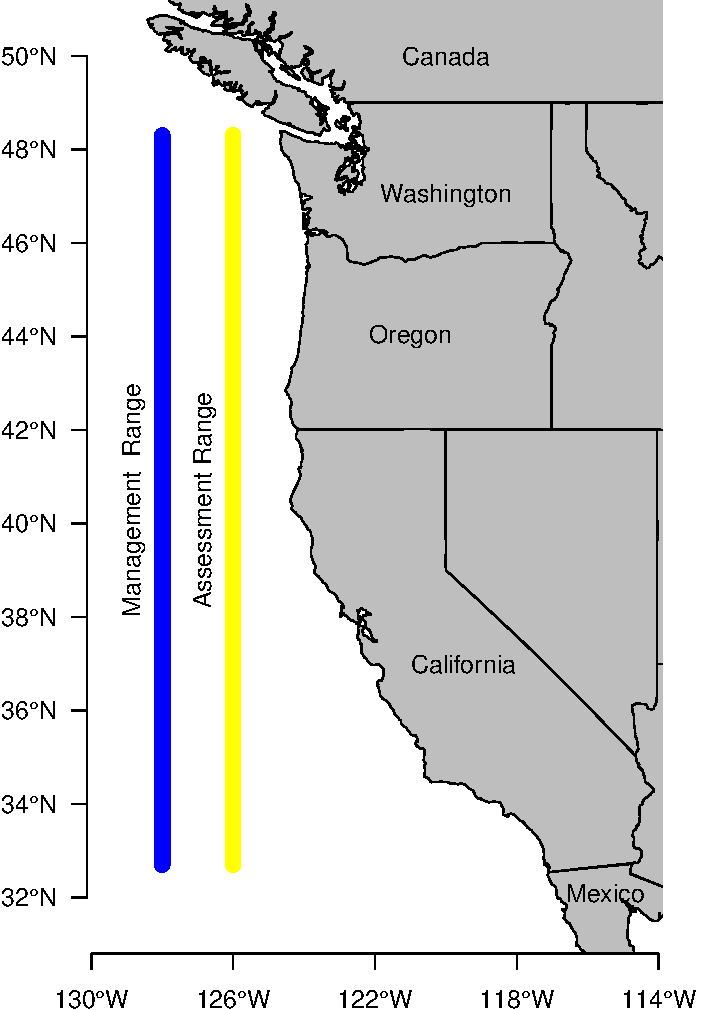
\includegraphics{SAR_USWC_Rougheye_and_Blackspotted_Rockfishes_skeleton_files/figure-pdf/fig-map-1.pdf}

}

\caption{\label{fig-map}Map of the assessment area.}

\end{figure}%

\begin{figure}

\centering{

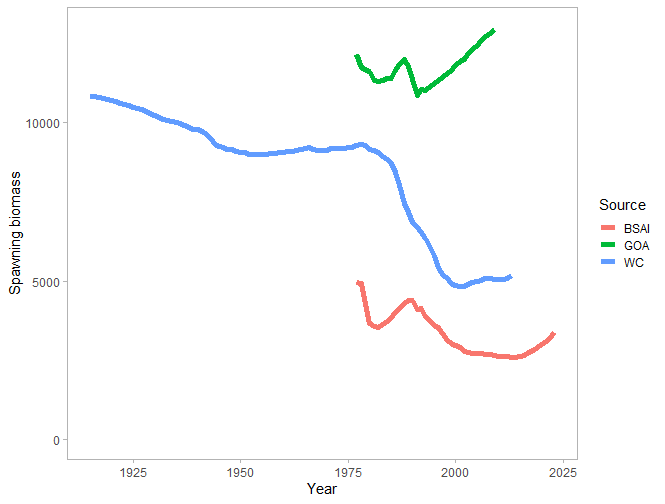
\includegraphics{plots_4_doc/SB_comps.png}

}

\caption{\label{fig-SO_comp}Estimates of spawning biomass (current
spawning output/unfished spawning output) for the Rougheye/Blackspotted
rockfish complex from the two most recent Alaska (Bering Sea/Aleutian
Islands (BSAI) and Gulf of Alaska (GOA)) and the 2013 U.S. west coast
stock assessment.}

\end{figure}%

\begin{figure}

\centering{

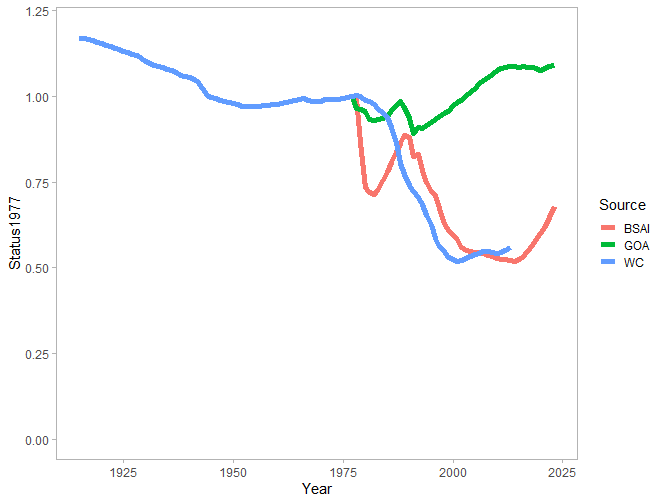
\includegraphics{plots_4_doc/Status_comp.png}

}

\caption{\label{fig-RSS_comp}Estimates of relative stock size (current
spawning output/unfished spawning output) relative to 1977 (the common
year in all stock assessments compared) for the Rougheye/Blackspotted
rockfish complex from the two most recent Alaska (Bering Sea/Aleutian
Islands (BSAI) and Gulf of Alaska (GOA)) and the 2013 U.S. west coast
stock assessment.}

\end{figure}%

\begin{figure}

\centering{

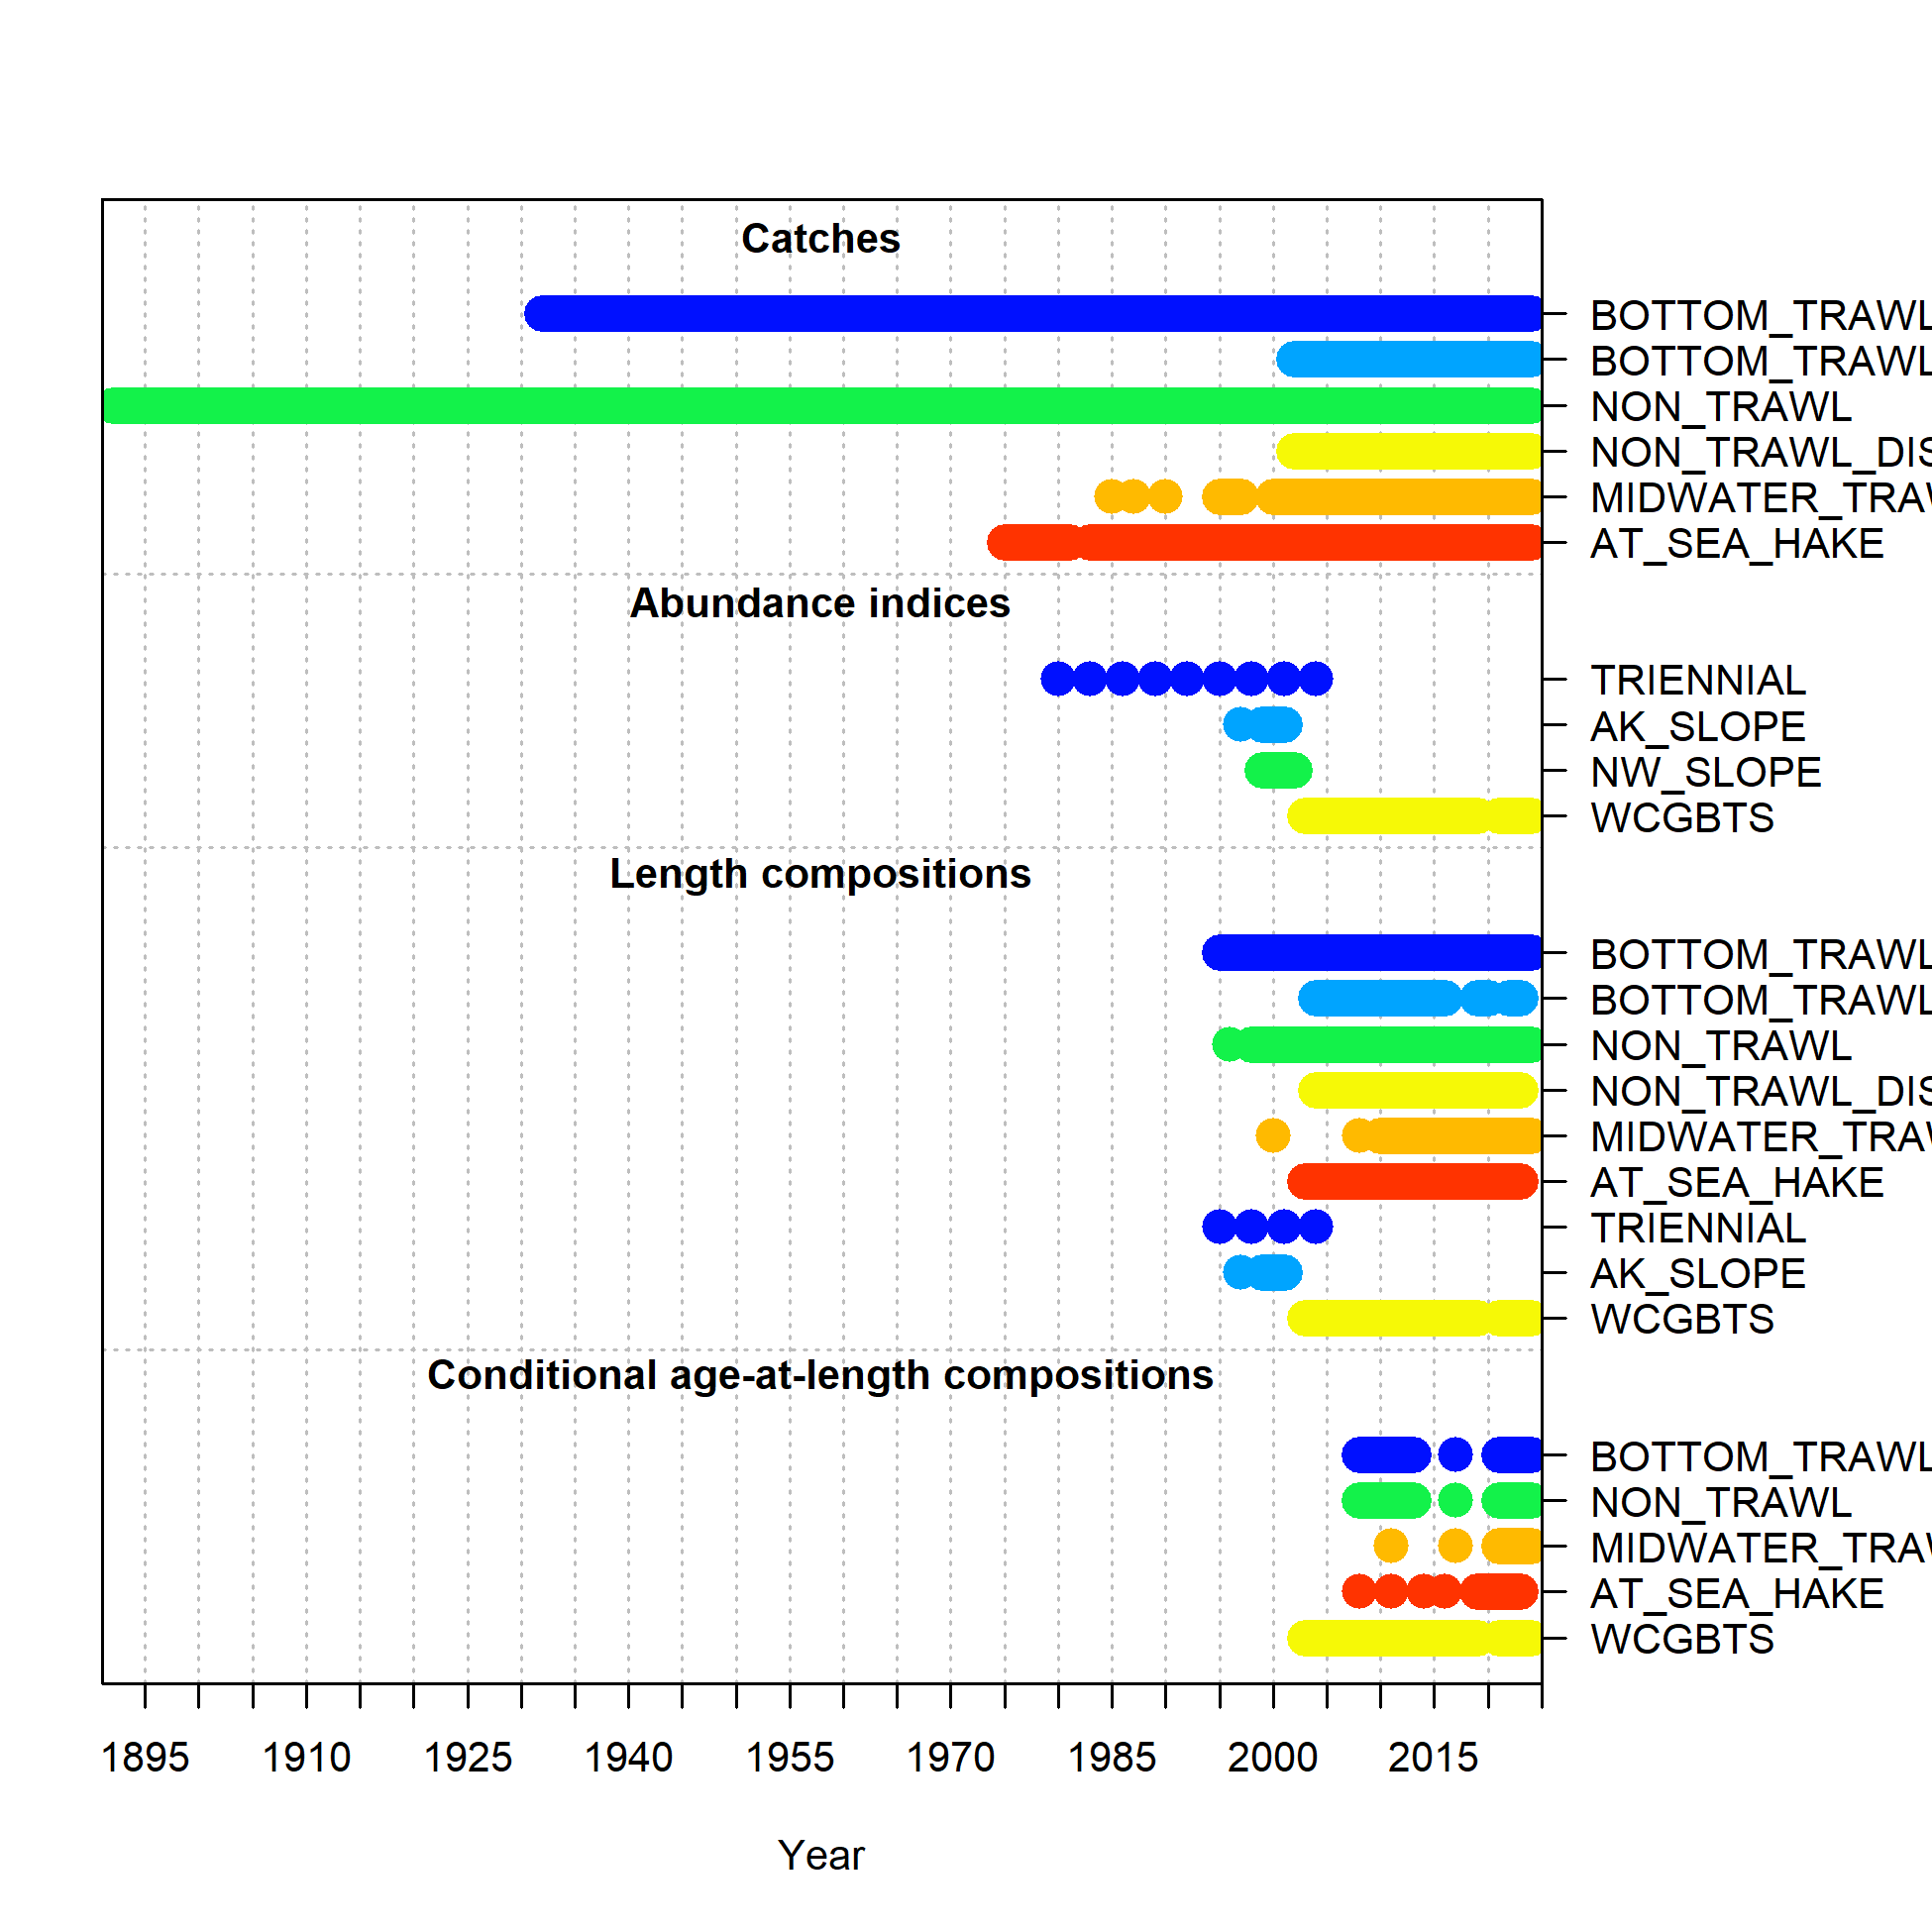
\includegraphics{ref_model/plots/data_plot.png}

}

\caption{\label{fig-data}Data used in the base model.}

\end{figure}%

\begin{figure}

\centering{

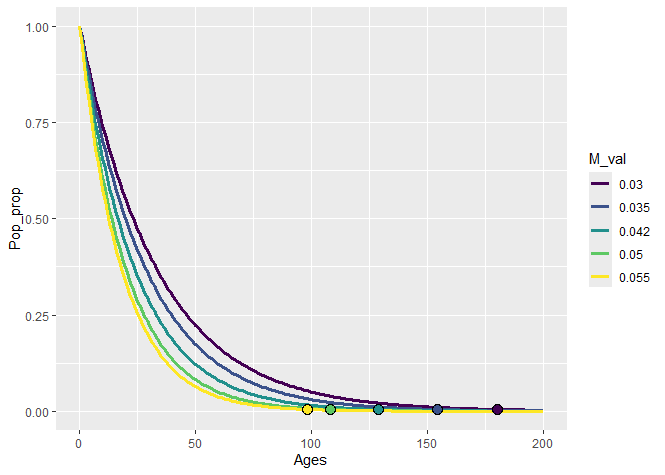
\includegraphics{plots_4_doc/M_values.png}

}

\caption{\label{fig-Mcurves}Natural mortality curves by age in years for
values of natural mortality used in various Rougheye/Blackspotted
Rockfish stock assessments. Dots indicate the range of assumed maximum
ages using the equation from Hamel and Cope 2022.}

\end{figure}%

\begin{figure}

\centering{

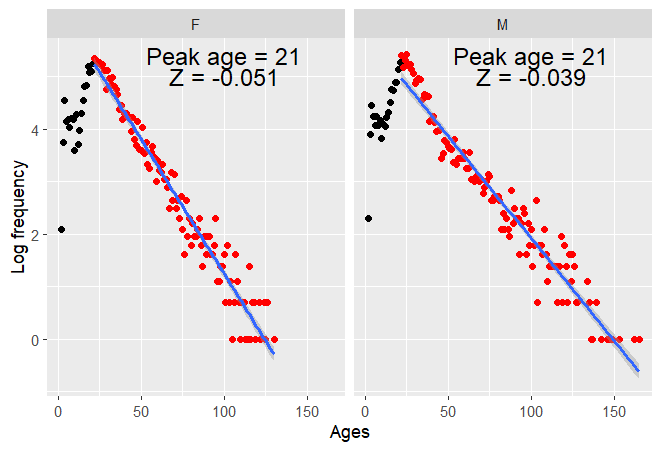
\includegraphics{plots_4_doc/Catch_curve_plot_FM.png}

}

\caption{\label{fig-CC_Z}Catch curve (log abundance by age) analysis on
aggregated ages over all age sources by sex (black points). The peak
selected age was 21 for both sexes, so the linear model was run from age
21 until the oldest age (red points). The slope of the linear model is
equal to the estimate of an aggregate total mortality (Z).}

\end{figure}%

\begin{figure}

\centering{

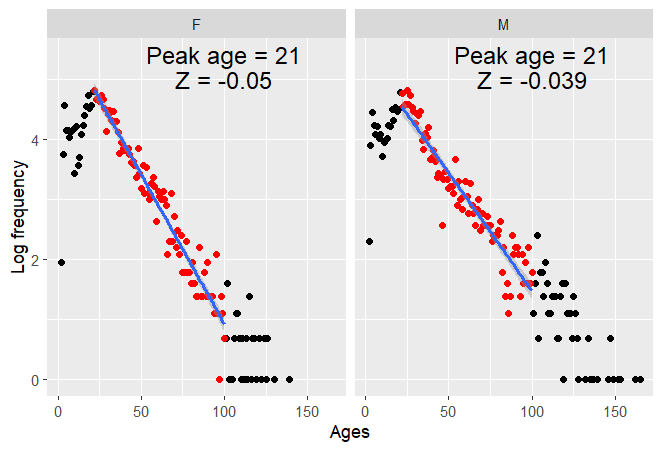
\includegraphics{plots_4_doc/Catch_curve_plot_FM_21_100.png}

}

\caption{\label{fig-CC_Z_100}Catch curve (log abundance by age) analysis
on aggregated ages over all age sources by sex (black points). The peak
selected age was 21 for both sexes with a max age of 100, so the linear
model was run from age 21 until age 100 (red points). The slope of the
linear model is equal to the estimate of an aggregate total mortality
(Z).}

\end{figure}%

\begin{figure}

\centering{

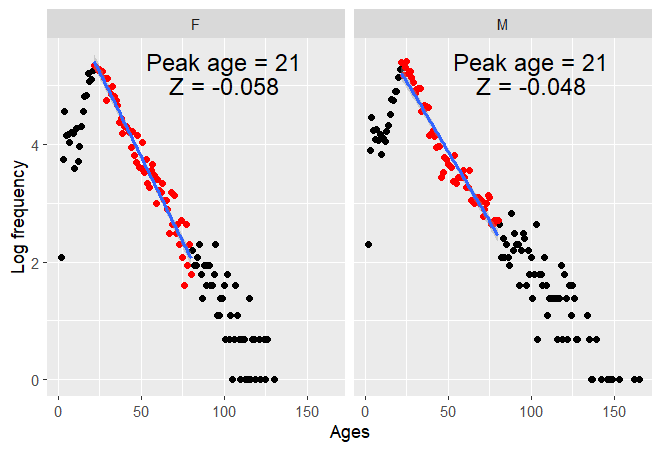
\includegraphics{plots_4_doc/Catch_curve_plot_FM_21_80.png}

}

\caption{\label{fig-CC_Z_80}Catch curve (log abundance by age) analysis
on aggregated ages over all age sources by sex (black points). The peak
selected age was 21 for both sexes with a max age of 80, so the linear
model was run from age 21 until age 80 (red points). The slope of the
linear model is equal to the estimate of an aggregate total mortality
(Z).}

\end{figure}%

\begin{figure}

\centering{

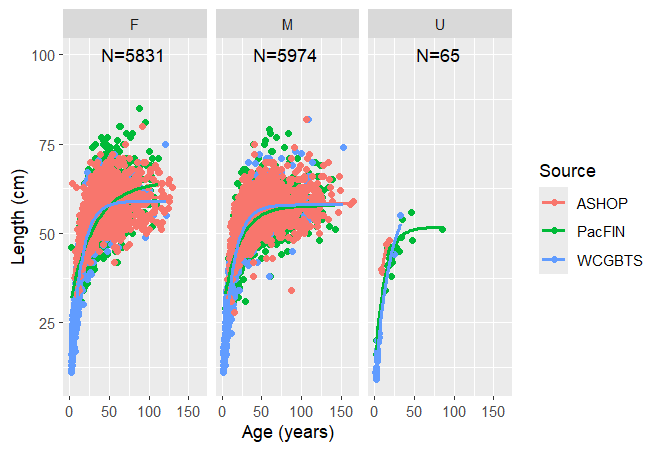
\includegraphics{plots_4_doc/Age_length_plot.png}

}

\caption{\label{fig-AL_1}Age and length data, with fitted von
Bertalanffy growth curves, by sex and data source for the
Rougheye/Blackspotted rockfish complex. Sample sizes (N) are also
provided.}

\end{figure}%

\begin{figure}

\centering{

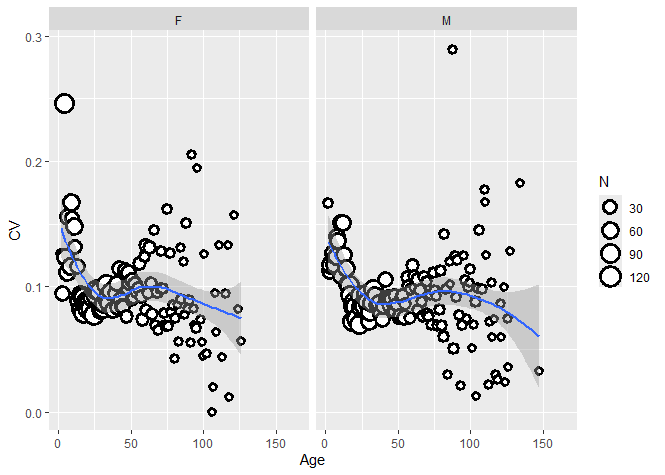
\includegraphics{plots_4_doc/Lt_age_CV_FM.png}

}

\caption{\label{fig-AL_2}Coefficient of variation by age and sex for all
sources of Rougheye/Blackspotted rockfishes ages. Sample sizes (N) are
also indicated by size of the point. The line is a smoothed loess
(polynomial) line that gives a moving average of CV by age and sex.}

\end{figure}%

\begin{figure}

\centering{

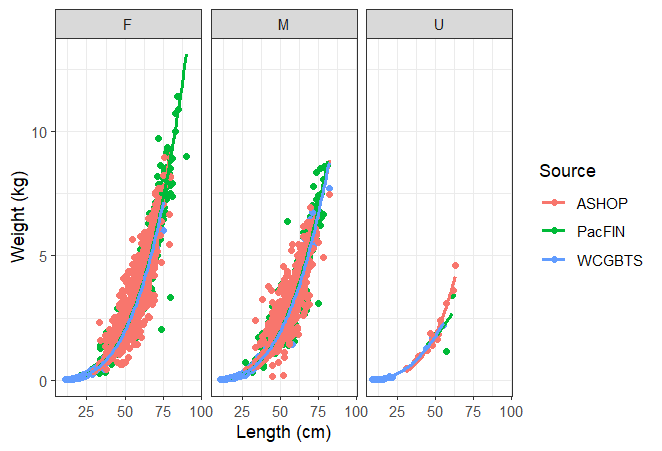
\includegraphics{plots_4_doc/L_W_plots.png}

}

\caption{\label{fig-LW1}Length and weight samples by sex and data
source. Lines are the power function fits by data source.}

\end{figure}%

\begin{figure}

\centering{

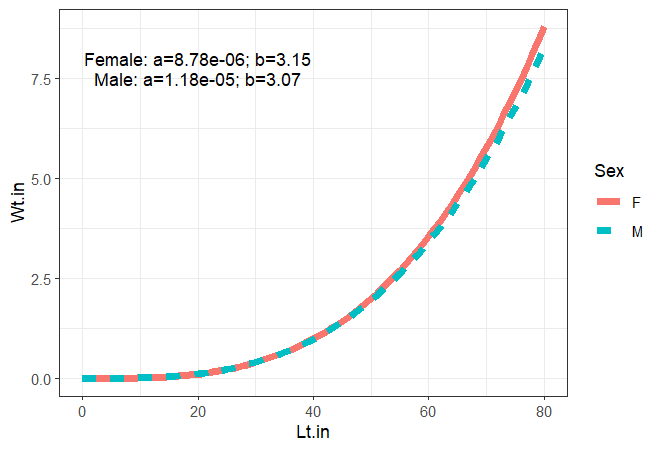
\includegraphics{plots_4_doc/F_M_ltwt_plot.png}

}

\caption{\label{fig-LW2}Realized length and weight relationships for
female and male Rougheye/Blackspotted Rockfishes.}

\end{figure}%

\begin{figure}

\centering{

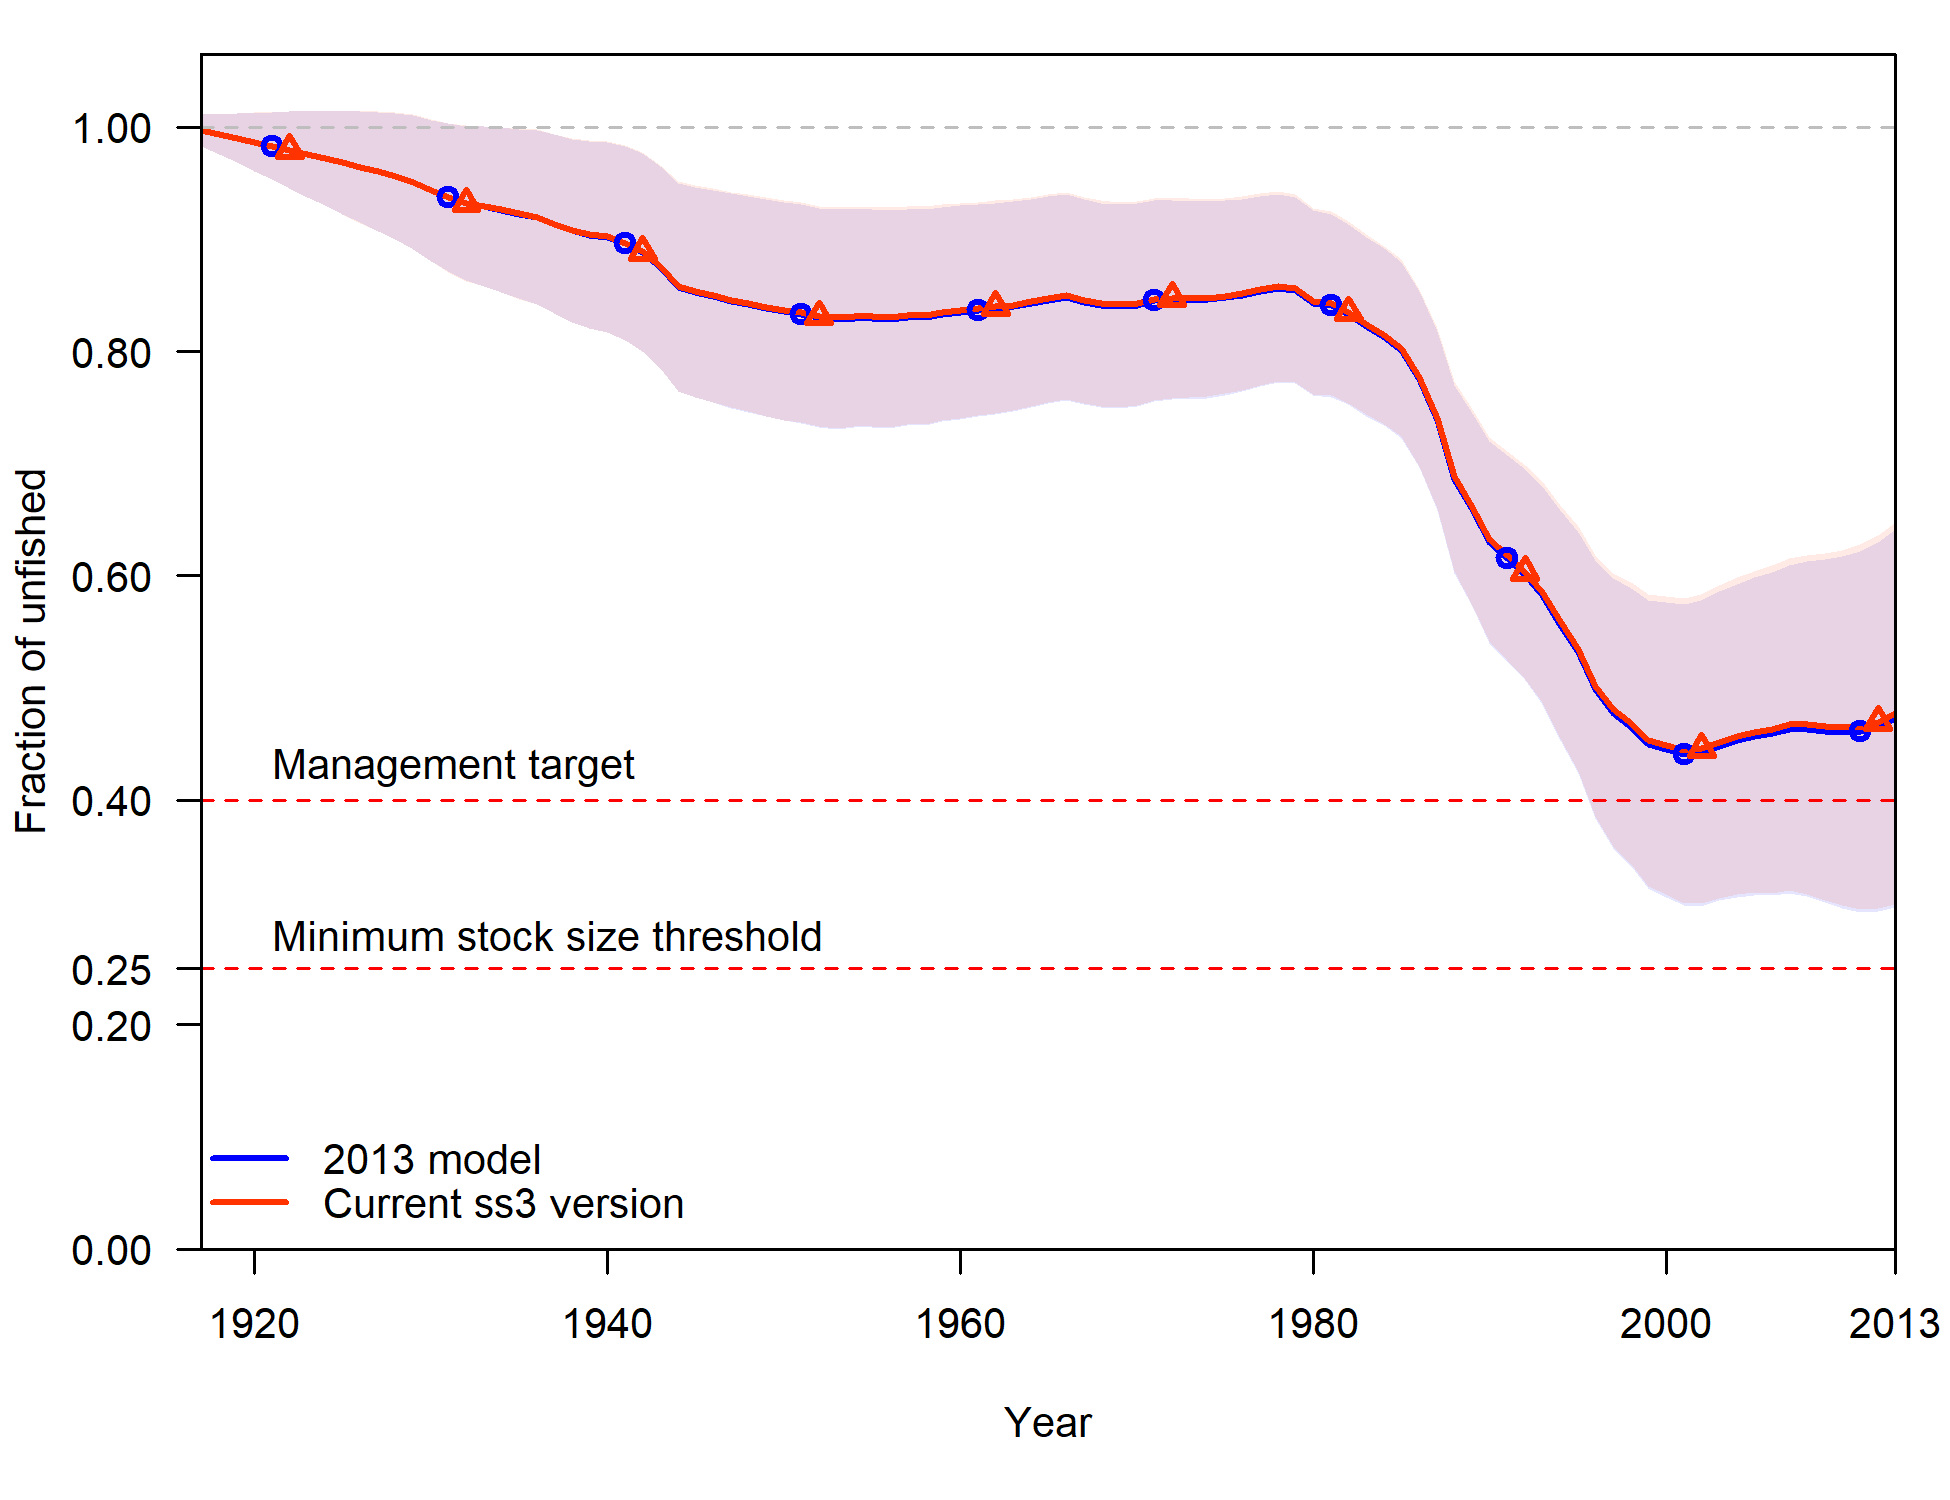
\includegraphics{plots_4_doc/compare4_Bratio_uncertainty.png}

}

\caption{\label{fig-RSS_2013}Estimates of relative stock size (current
spawning output/unfished spawning output) for the Rougheye/Blackspotted
rockfish complex in U.S. west coast waters from the 2013 assessment, and
compared to the using the same data in the newest version of SS3
(3.330.22.1).}

\end{figure}%

\begin{figure}

\centering{

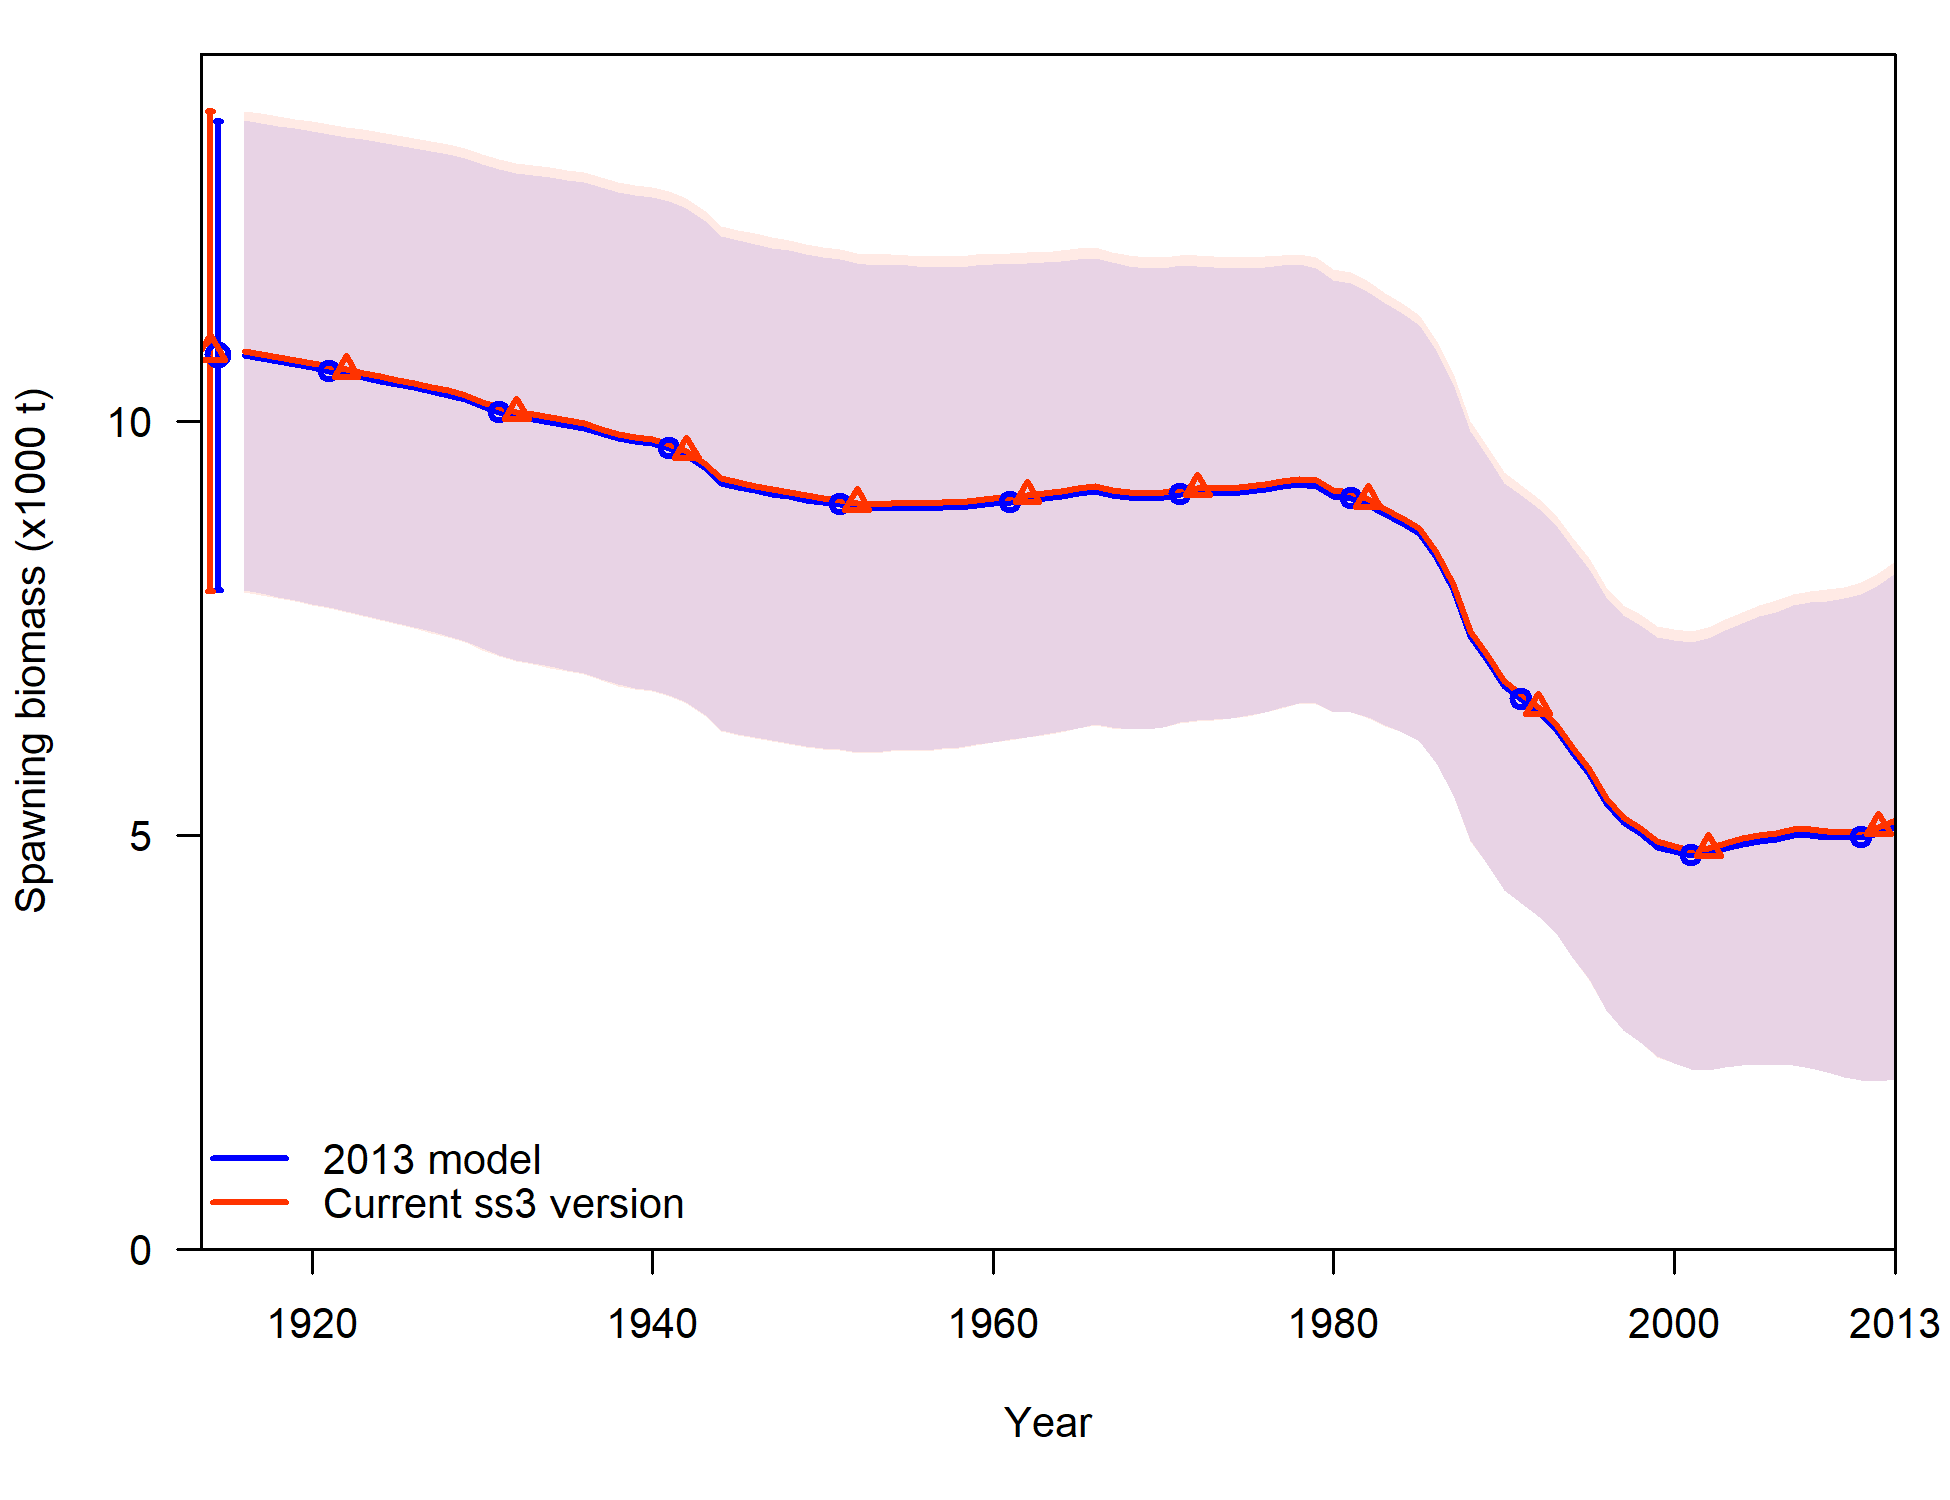
\includegraphics{plots_4_doc/compare2_spawnbio_uncertainty.png}

}

\caption{\label{fig-SO_2013}Estimates of spawning output for the
Rougheye/Blackspotted rockfish complex in U.S. west coast waters from
the 2013 assessment, and compared to the same data in the newest version
of SS3 (3.330.22.1). Shading denotes 95\% confidence intervals. Shading
denotes 95\% confidence intervals.}

\end{figure}%

\begin{figure}

\centering{

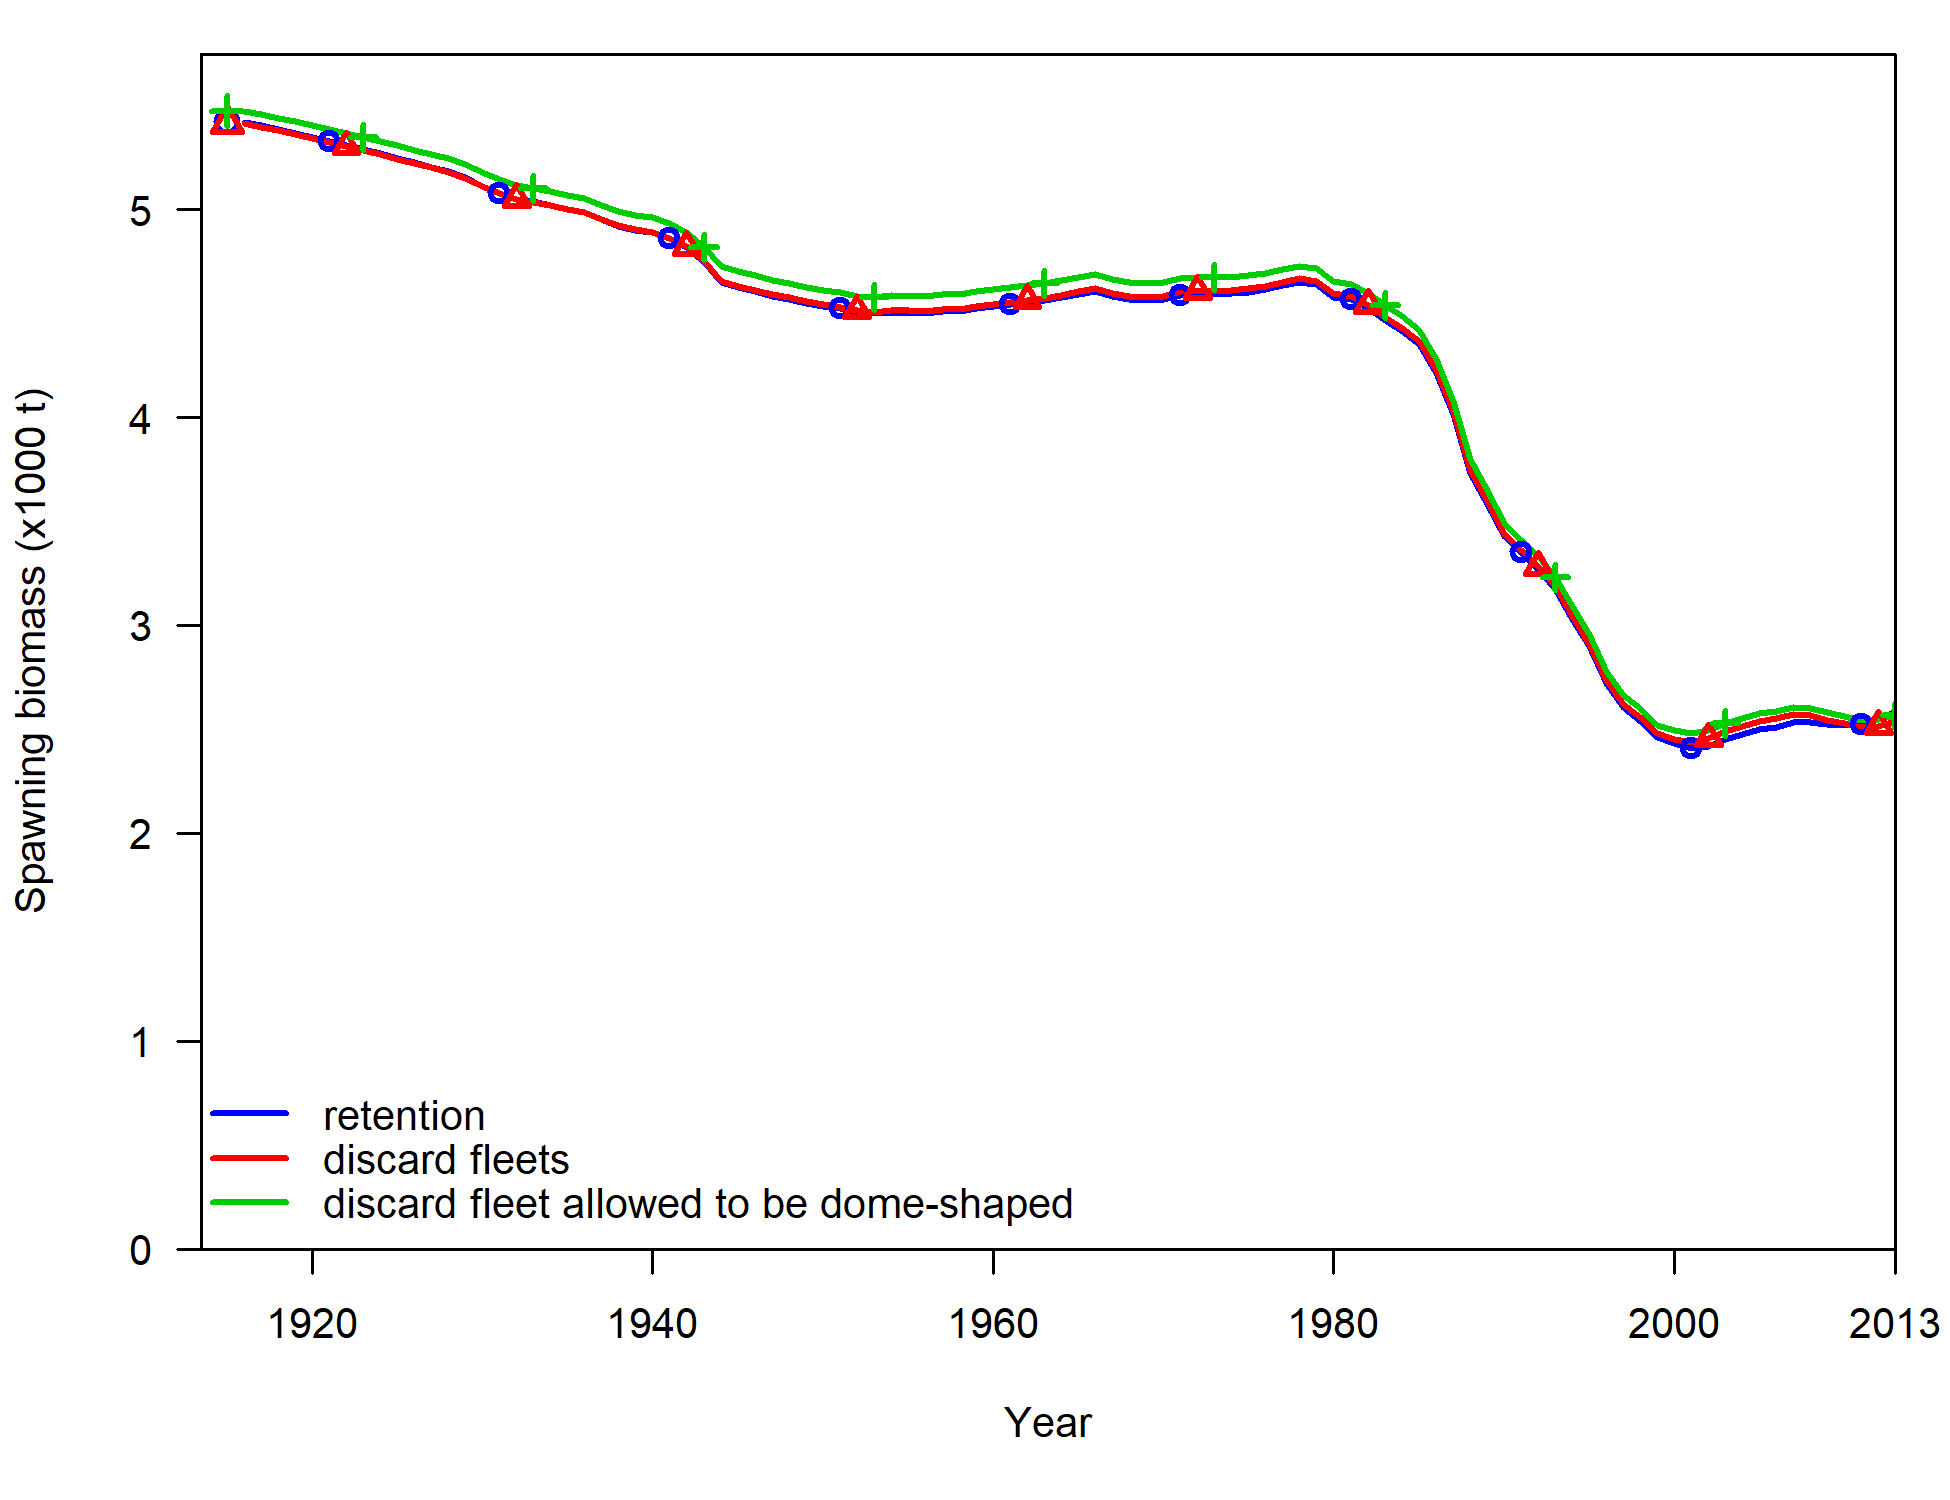
\includegraphics{plots_4_doc/compare1_spawnbio__discard_fleets.png}

}

\caption{\label{fig-Discard_comp_SO}Comparison of spawning output using
retention curves or discard fleets using the 2013 Rougheye/Blackspotted
Rockfishes assessment.}

\end{figure}%

\begin{figure}

\centering{

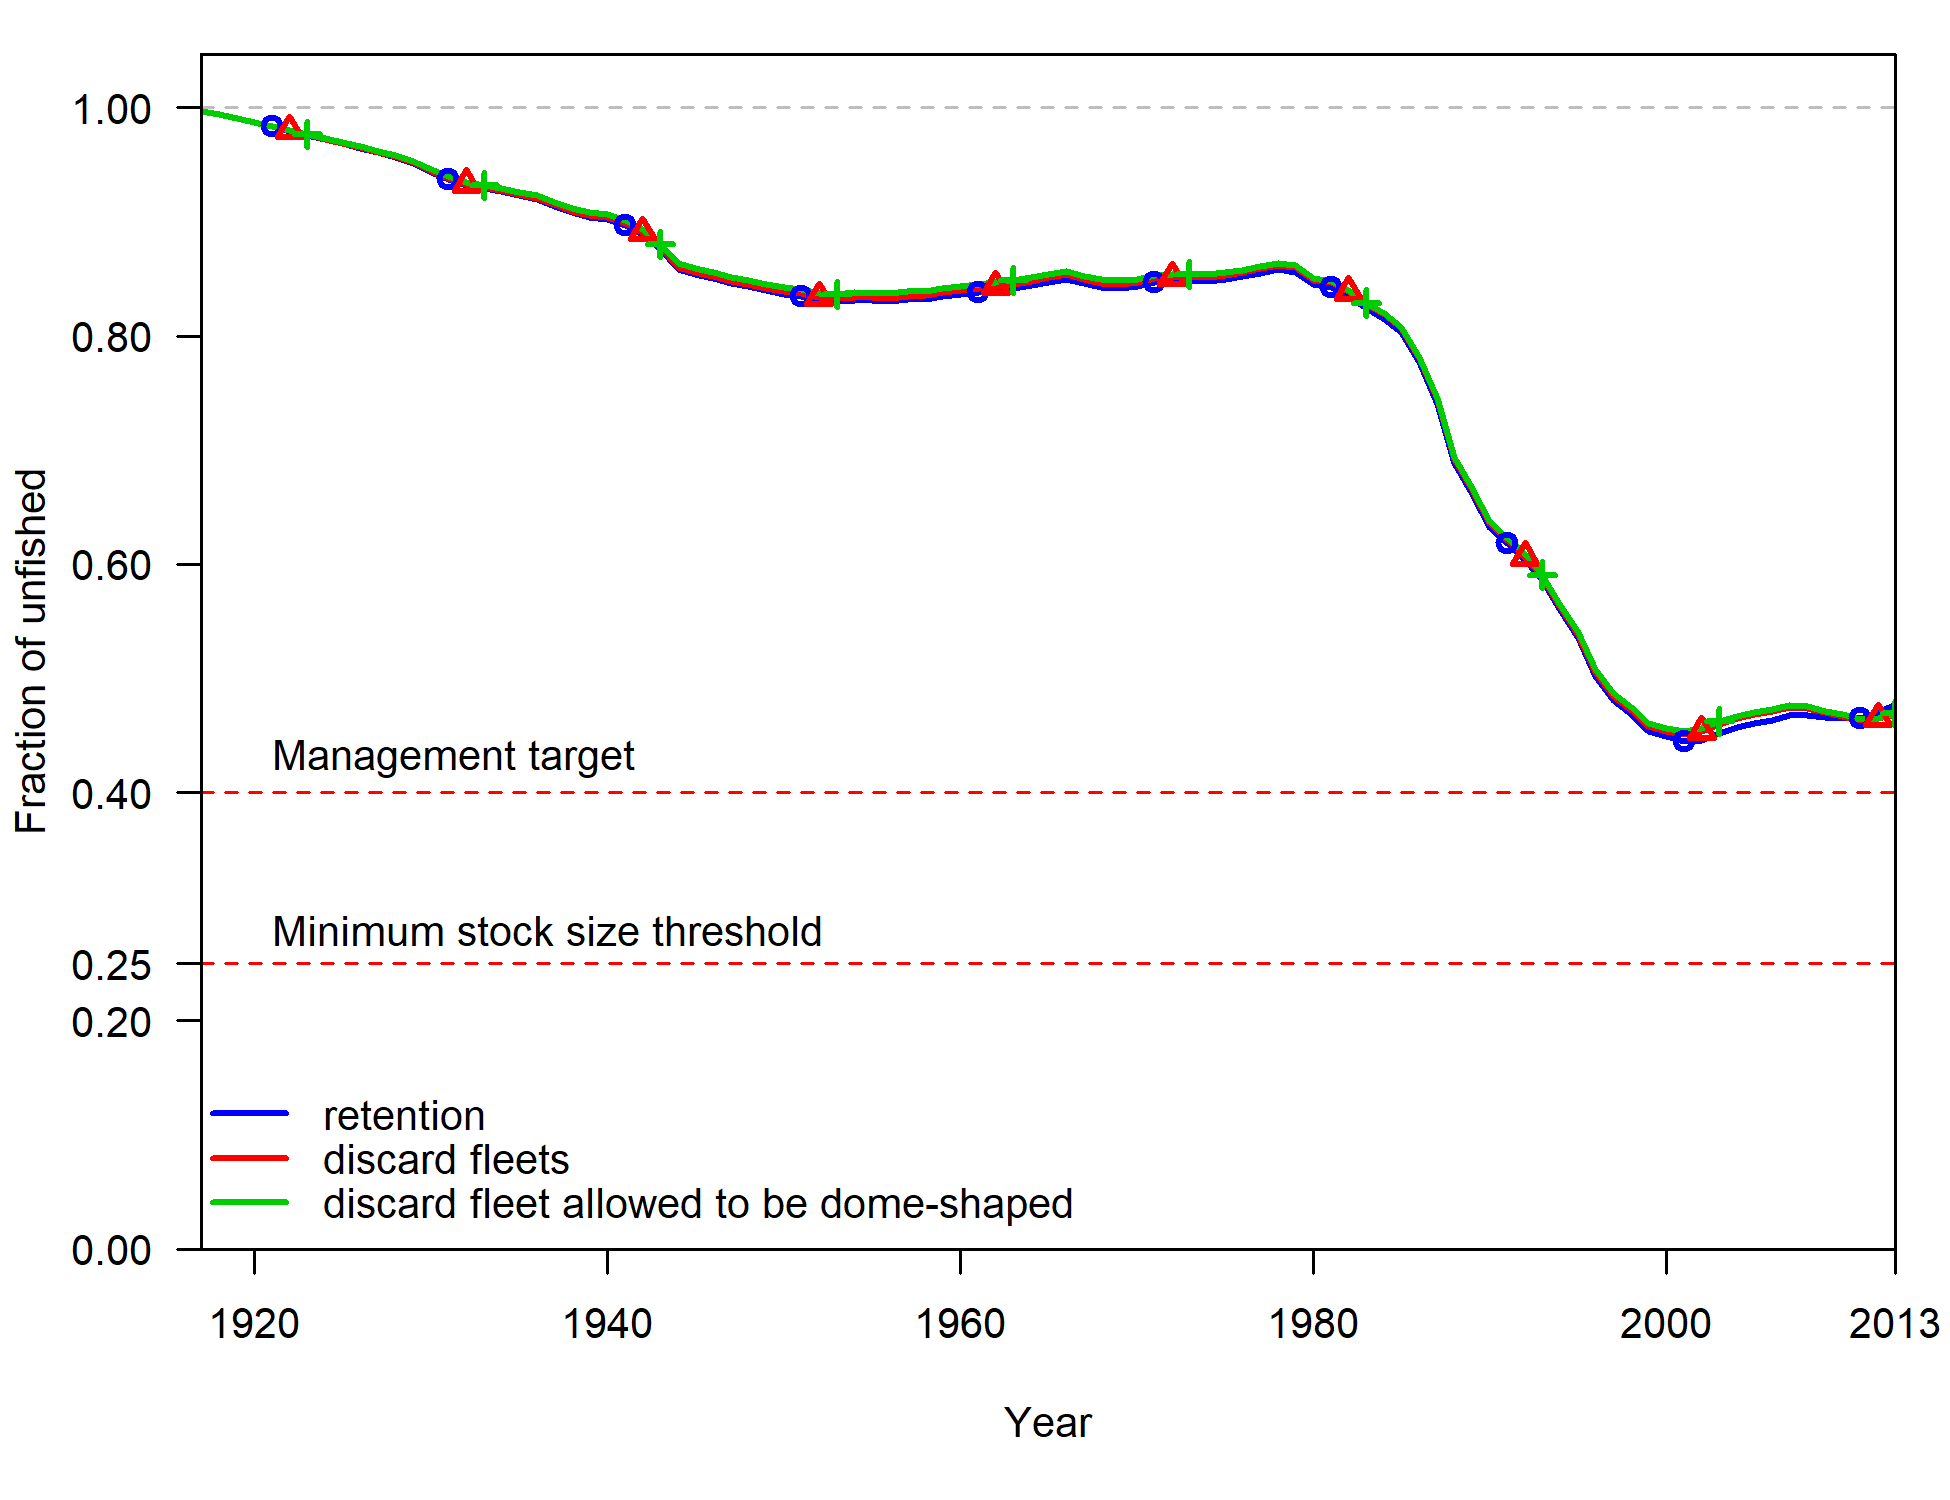
\includegraphics{plots_4_doc/compare3_Bratio_discard_fleets.png}

}

\caption{\label{fig-Discard_comp_RSS}Comparison of relative spawning
output using retention curves or discard fleets using the 2013
Rougheye/Blackspotted Rockfishes assessment.}

\end{figure}%

\newpage{}

\subsection{Notes}\label{notes}

\newpage{}

\subsection{Appendices}\label{sec-appendix}




\end{document}
